\documentclass[aspectratio=169]{beamer}
\usetheme{metropolis}  

\metroset{block=fill}

\setlength{\parindent}{0pt}
\usepackage[utf8]{inputenc}
\usepackage{amsbsy}
\usepackage{amsmath}
\usepackage{enumitem}
\usepackage{hyperref}
\usepackage{array}
\usepackage[T1]{fontenc}
\usepackage{tikz}
\usepackage{latexsym,xcolor,multicol,booktabs,calligra}
\usepackage{amsmath,amssymb,BOONDOX-cal,bm}	
\usepackage{graphicx,stackengine}   
\usepackage{xcolor}
\usepackage[sfdefault]{AlegreyaSans}
\usepackage{tabularx} 

\definecolor{white}{RGB}{255,255,255}
\setbeamercolor{background canvas}{bg=white}
\setbeamercolor{normal text}{bg=white}

\title{Causal Inference Project:\\ Impact of Scholarships on Student Success}
\date{April 04th, 2025}
\author{Anushka Mukherjee, Lucie Marimar, Jort Koks, Jakob Sarrazin}
\institute{Machine Learning for Econometrics \\ ENSAE, IP Paris \\ Bruno Crépon, Matthieu Doutreligne}

% ---------------------------------------
% Begin Document
% ---------------------------------------

\begin{document}
  \maketitle
  
% ---------------------------------------
% Section Motivation
% ---------------------------------------

   \section{1. Motivation}
  
  \begin{frame}{Motivation I}
  		\begin{columns}
	\begin{column}{0.7\textwidth}
	\textbf{Retention and Completion: A Core Challenge for Universities}

  		\begin{itemize}
  		\item [$\rightarrow$] \textbf{High dropout rates} are a persistent issue in higher education, especially during the first years of study.
  		\item [$\rightarrow$] \textbf{Timely graduation} is crucial for both students (career entry) and universities (funding, reputation
  		\item [$\Rightarrow$] \textbf{Financial constraints} are a major barrier to academic success — especially for socio-economically disadvantaged students.
  	\end{itemize}
  \end{column}

	\begin{column}{0.3\textwidth}
	\begin{center}
     
\includegraphics[width=1\textwidth]{Tex_Pictures/hat.png}
     \end{center}
	\end{column}

\end{columns}

  	
  \end{frame}
  
  \begin{frame}{Motivation II}
  	\textbf{Scholarships as a Tool to Improve Student Retention and Graduation}
  	
  	\begin{itemize}
  		\item [$\rightarrow$]  \textbf{Scholarship programs} are widely used as an intervention, but:
  		\begin{itemize}
  		  		\item [--] Their  \textbf{causal effect} on student outcomes is difficult to measure
  		  		\item [--] Many studies show correlations, but few rigorously identify causality.
   		\end{itemize}
   		\item [$\rightarrow$] This study uses a \textbf{causal machine learning framework (DML)} to estimate the  \textbf{true effect of scholarships}, adjusting for observed confounders.
   		\item [$\rightarrow$] Findings can inform \textbf{policy decisions} on financial aid allocation and \textbf{targeting of support} for at-risk students.
  	\end{itemize}
  \end{frame}
  
% ---------------------------------------
% Section PICO & RQ
% ---------------------------------------
  
  \section{2. PICO \& Research Question}
  
  \begin{frame}{PICO Formulation}
  \textbf{Population, Intervention, Comparison, Outcome}
  	\begin{itemize}
  		\item [P - ] Undergraduate students at a Portuguese university (N = 4,424), with data on demographics, socio-economic background, and prior academic performance.
  		\item [I - ] Receiving a scholarship during university studies.
  		\item [C - ] Students without scholarships, adjusted for observed confounders (grades, family background, gender, etc.).
  		\item [O - ] Two binary outcomes observed 3 years after enrollment:
  
  	\begin{itemize}
  		\item [1.] Dropout vs. Enrolled/Graduated
  		\item [2.] Graduated vs. Dropout/Enrolled
  	\end{itemize}
  	
  	\end{itemize}
  \end{frame}

  
  \begin{frame}{Research Question}
    \begin{alertblock}{RQ1}
	Does receiving a scholarship \textbf{reduce} the likelihood of \textbf{dropping out} within 3 years?
\end{alertblock}
\vspace{10pt}
    \begin{alertblock}{RQ2}
	Does receiving a scholarship \textbf{increase} the likelihood of \textbf{graduating} within 3 years?
\end{alertblock}
  \end{frame}
  

\section{3. Data Overview and Exploratory Analysis}

\begin{frame}{The Data}
	\textbf{Source}
	\begin{itemize}
		\item [--] UCI Machine Learning Repository – Predict Students Dropout and Academic Success 
	\end{itemize}
	
	\textbf{Scope}
	\begin{itemize}
		\item [--] Administrative records from a Portuguese university $\rightarrow$ 4,424 undergraduate students across various degree programs
	\end{itemize}
	
	\textbf{Observation Period}
	\begin{itemize}
		\item [--] Students tracked for 3 years after enrollment.
	\end{itemize}
\end{frame}

\begin{frame}{Variables}
\centering
\renewcommand{\arraystretch}{1.4}

\begin{tabularx}{\textwidth}{X | X | X}
\textbf{Outcome Variable} & \textbf{Treatment Variable} & \textbf{Covariates}  (Pre Treatment)\\[0.5ex]
\hline \hline 
Student status after 3 years: 
\parbox[t]{4cm}{\vspace{-12pt} \begin{itemize}[label=--,leftmargin=1.2em,itemsep=1pt,topsep=2pt]
    \item Dropout
    \item Still enrolled
    \item Graduated
    \item[$\rightarrow$] \textit{Re-coded into two binary variables for RQ1 \& RQ2}
\end{itemize}} &

Received scholarship or not (\textit{Binary variable}) 

& \vspace{-27pt}
\parbox[t]{4cm}{\begin{itemize}[label=--,leftmargin=1.2em,itemsep=1pt,topsep=2pt]
    \item Academic performance before university
    \item Family background
    \item Economic context
    \item Demographics
\end{itemize}}

\end{tabularx}
\end{frame}

\begin{frame}{Outcome Variable}
	\begin{center}
     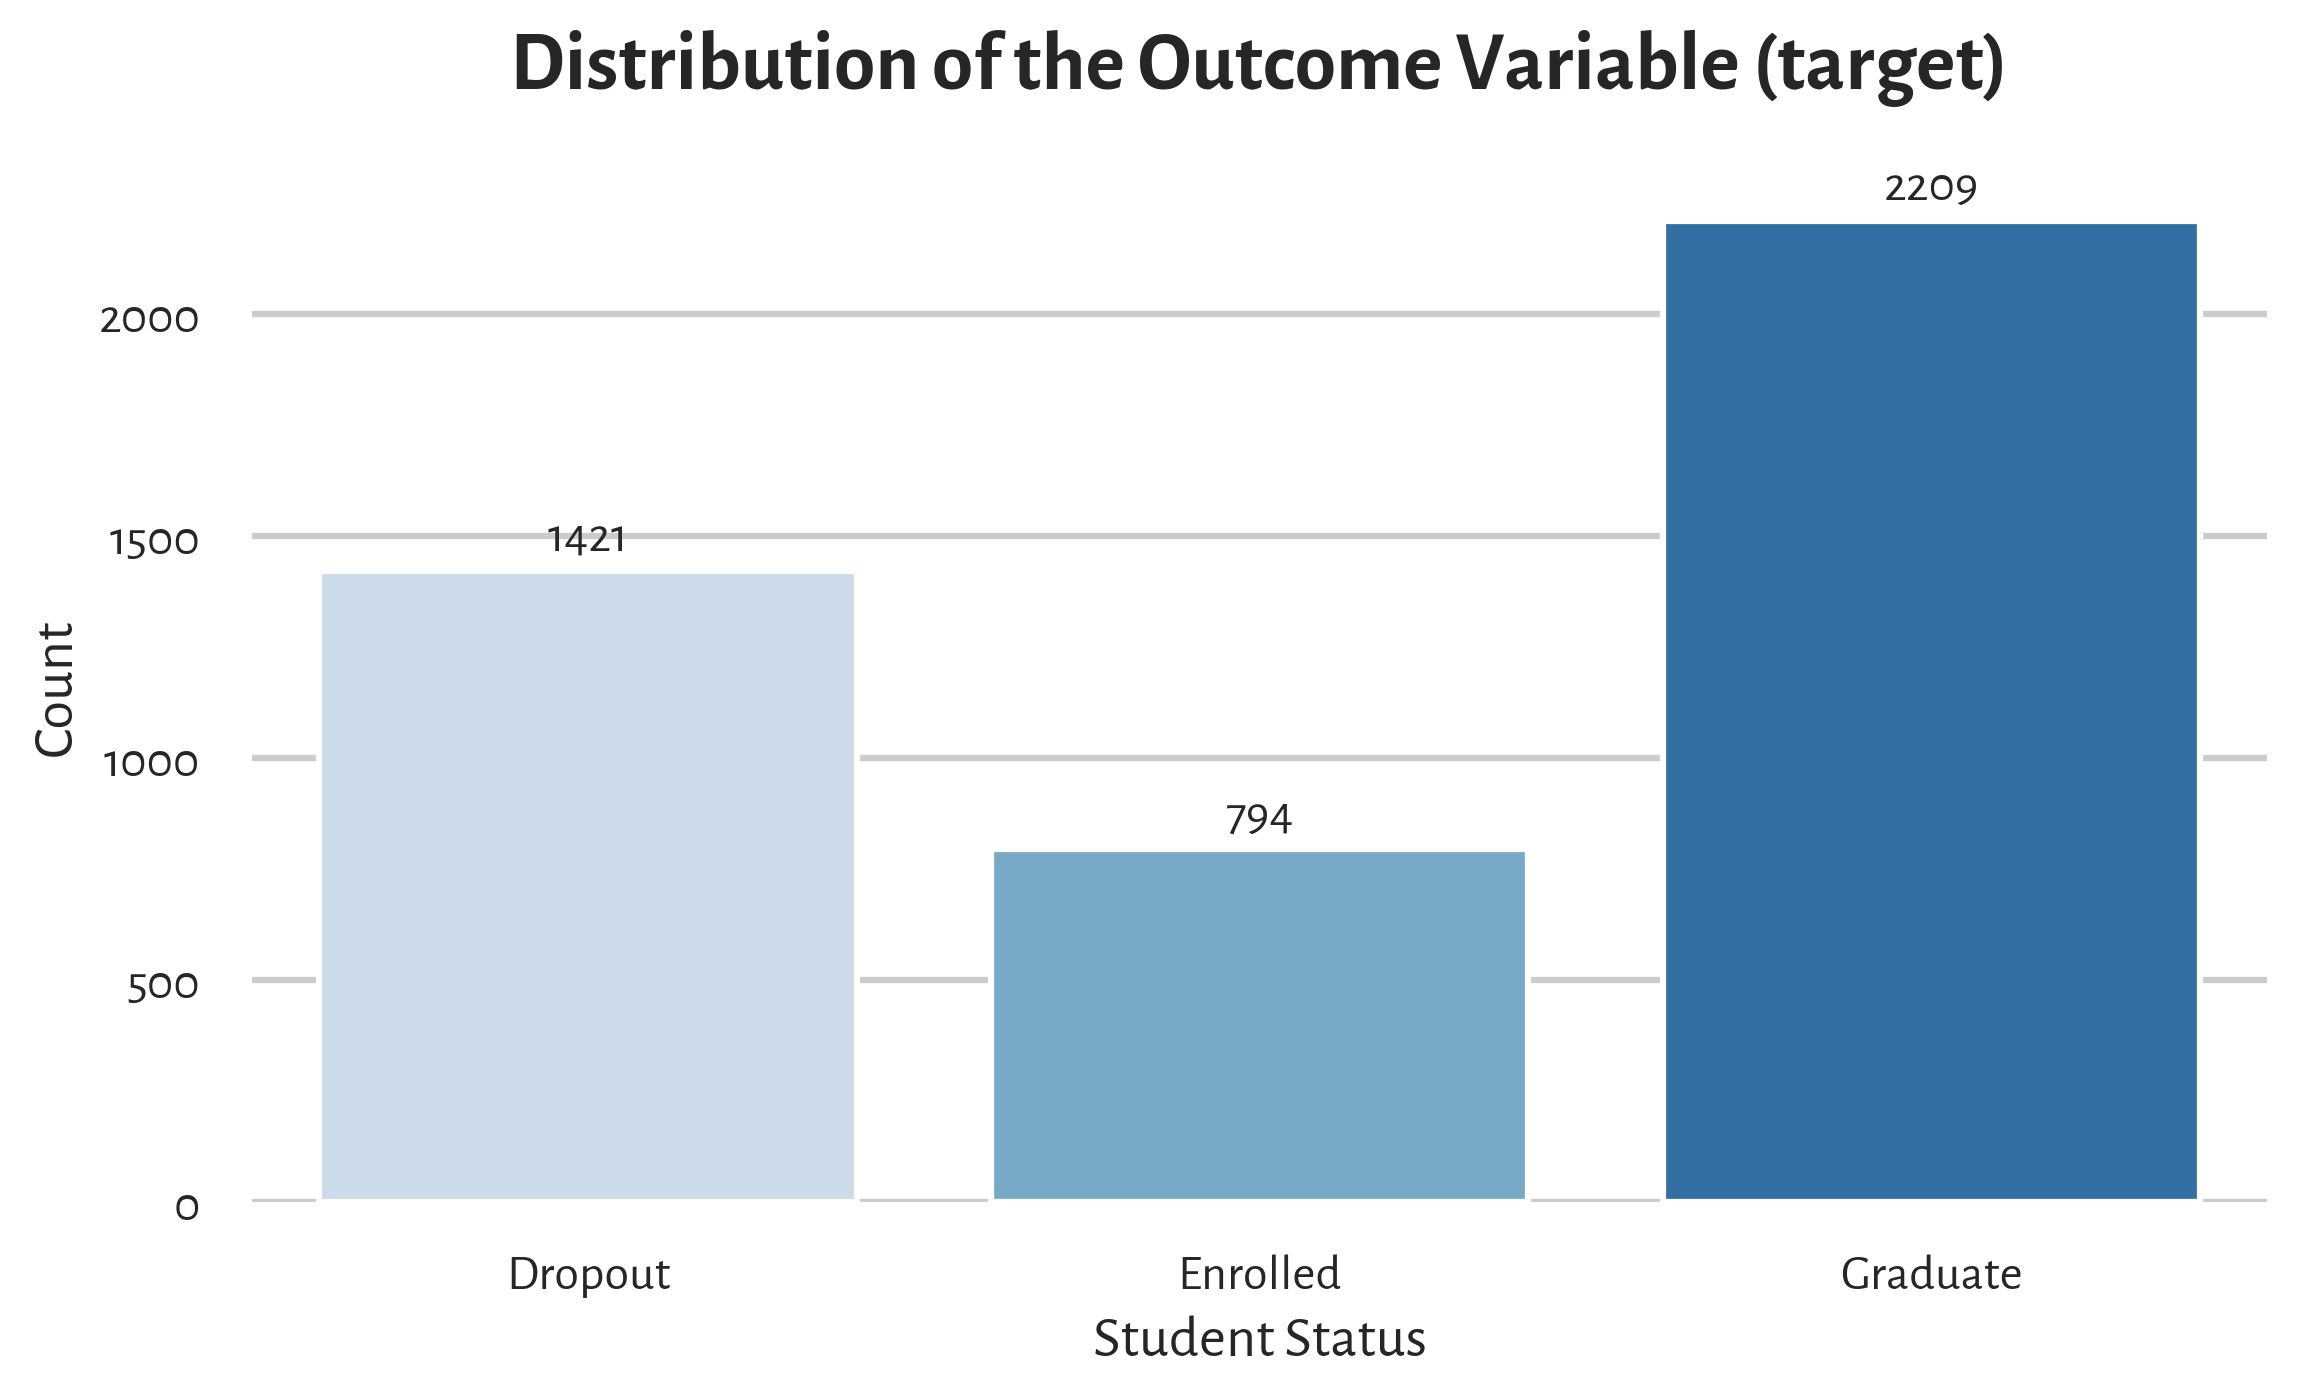
\includegraphics[width=0.85\textwidth]{Tex_Pictures/Graph1.png}
     \end{center}
\end{frame}

\begin{frame}{Treatment vs Outcome Variable}
	\begin{center}
     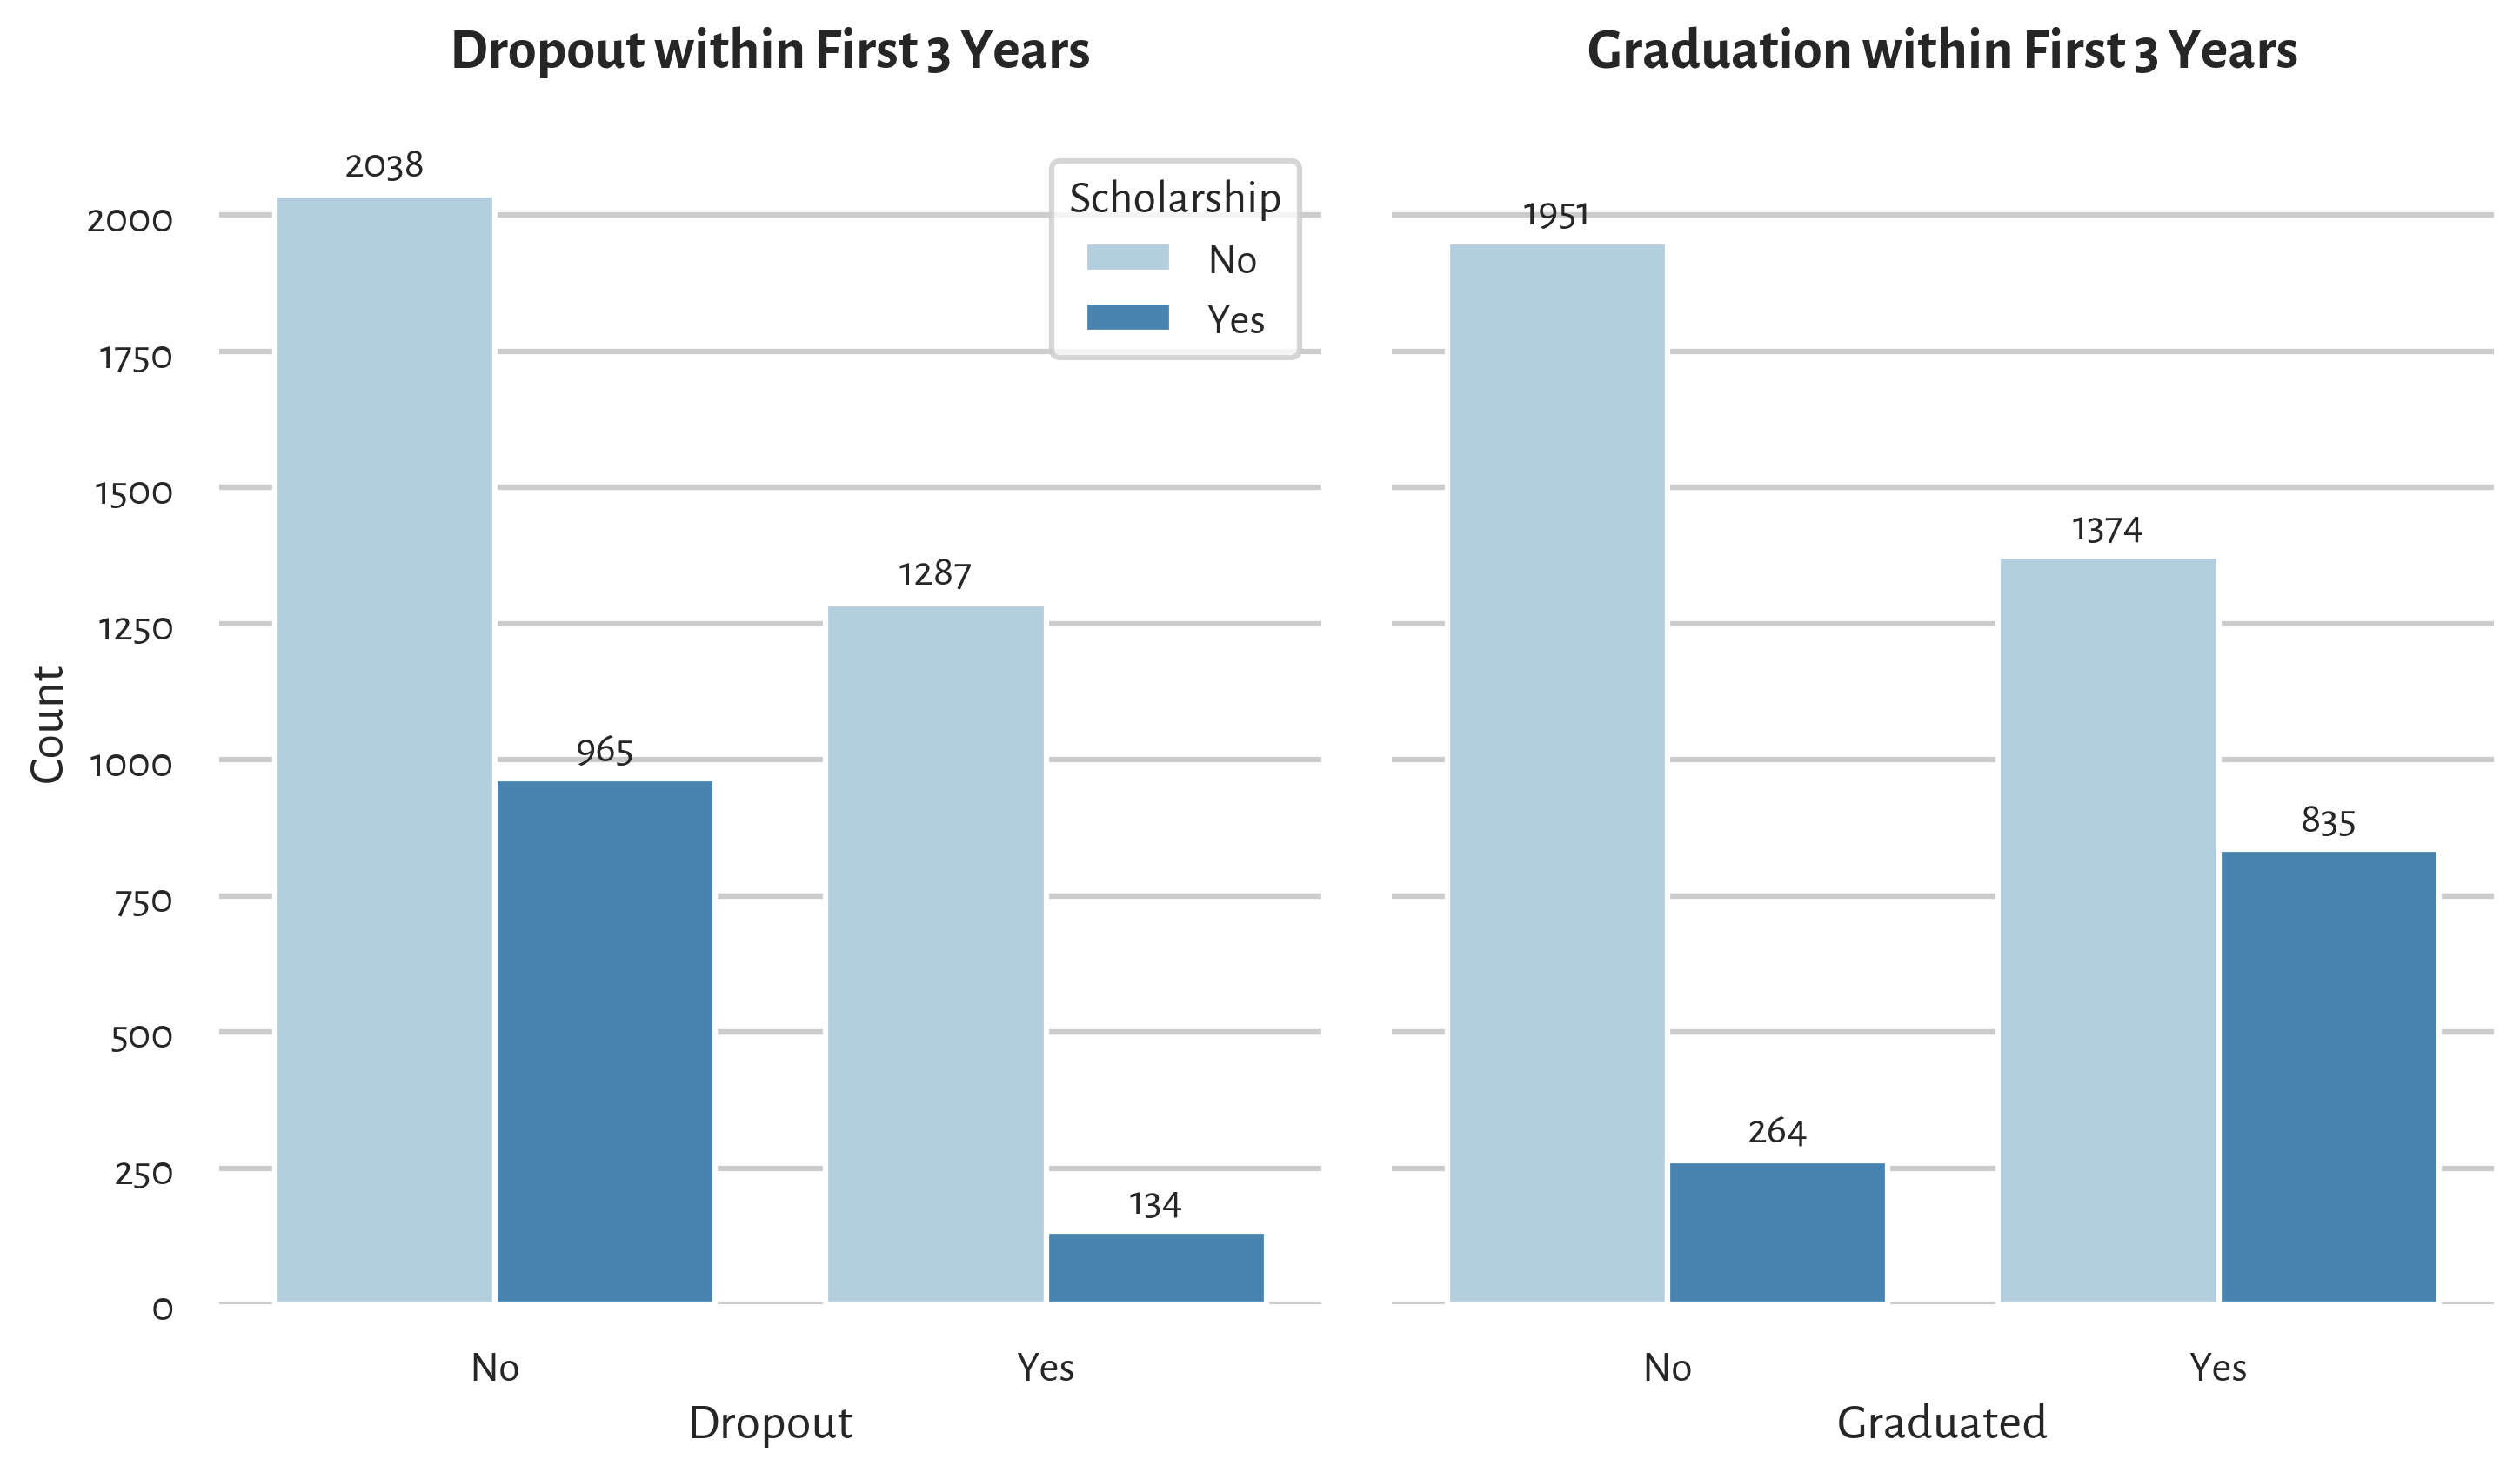
\includegraphics[width=0.8\textwidth]{Tex_Pictures/Graph2.png} \\
     \small
     Dropout (Graduation) probability decreases (increases) by 68.50\% (83.86\%) for scholarship holders.
     \end{center}
\end{frame}

\begin{frame}{Covariates: Academic Preperation}
	\begin{center}
     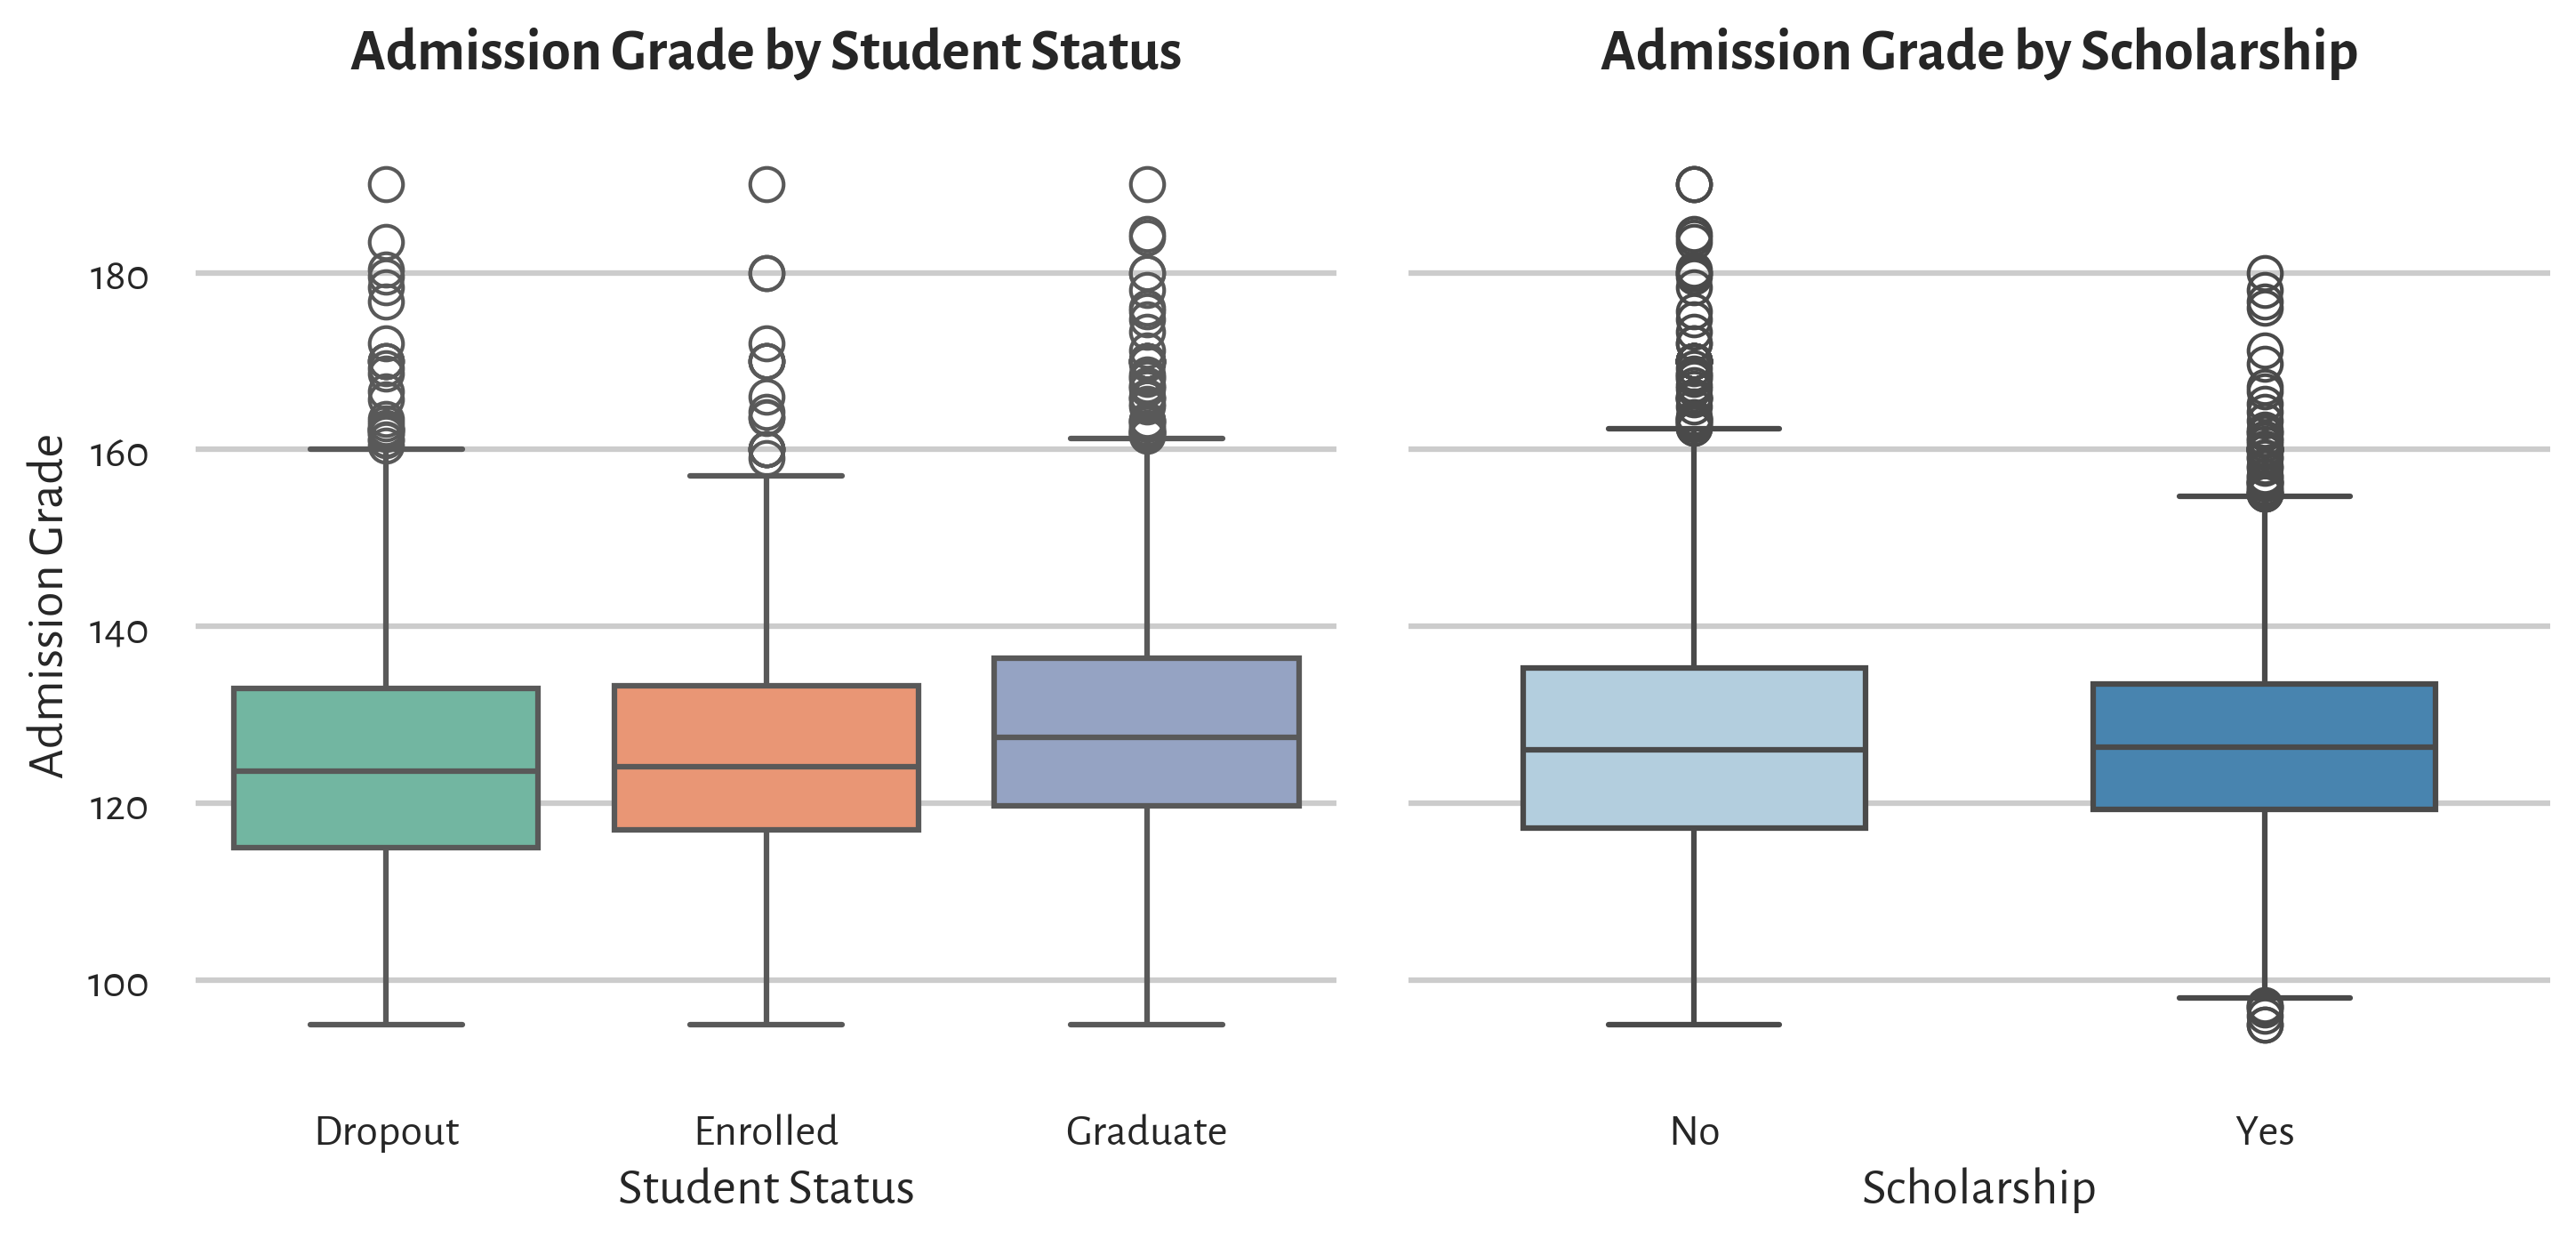
\includegraphics[width=1\textwidth]{Tex_Pictures/Graph_admission_grade.png} \\
     \end{center}
\end{frame}

\begin{frame}{Covariates: Family Background}
	\begin{center}
     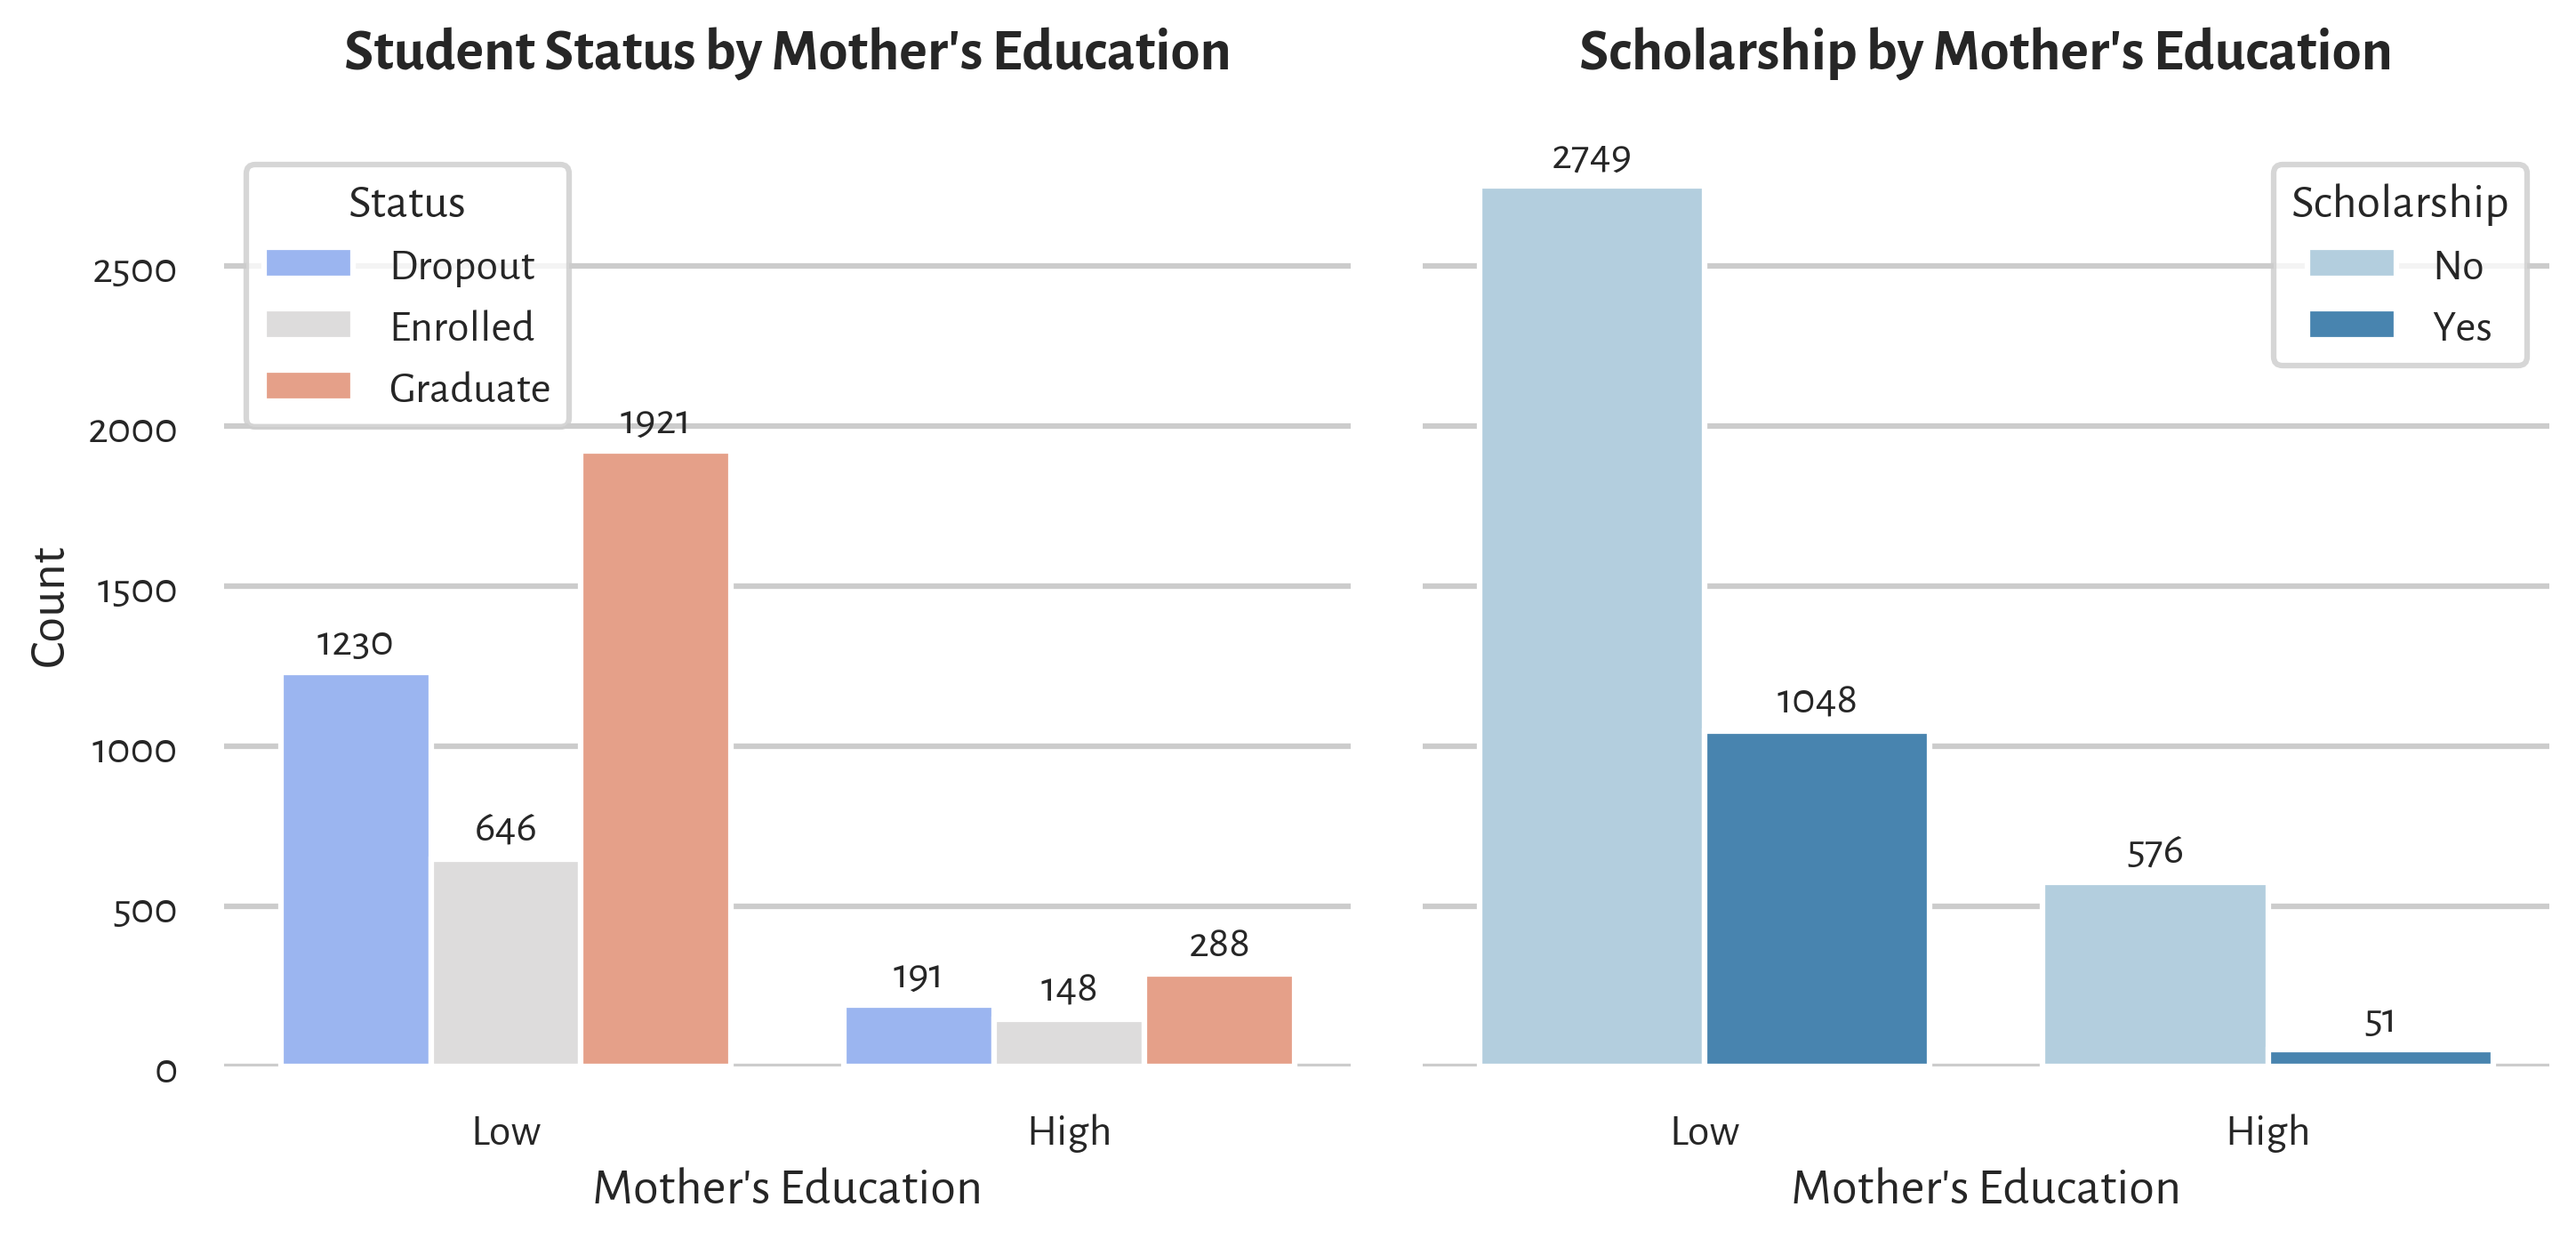
\includegraphics[width=1\textwidth]{Tex_Pictures/Graph_mother_educ}
     \end{center}
\end{frame}

\begin{frame}{Covariates: Gender}
	\begin{center}
     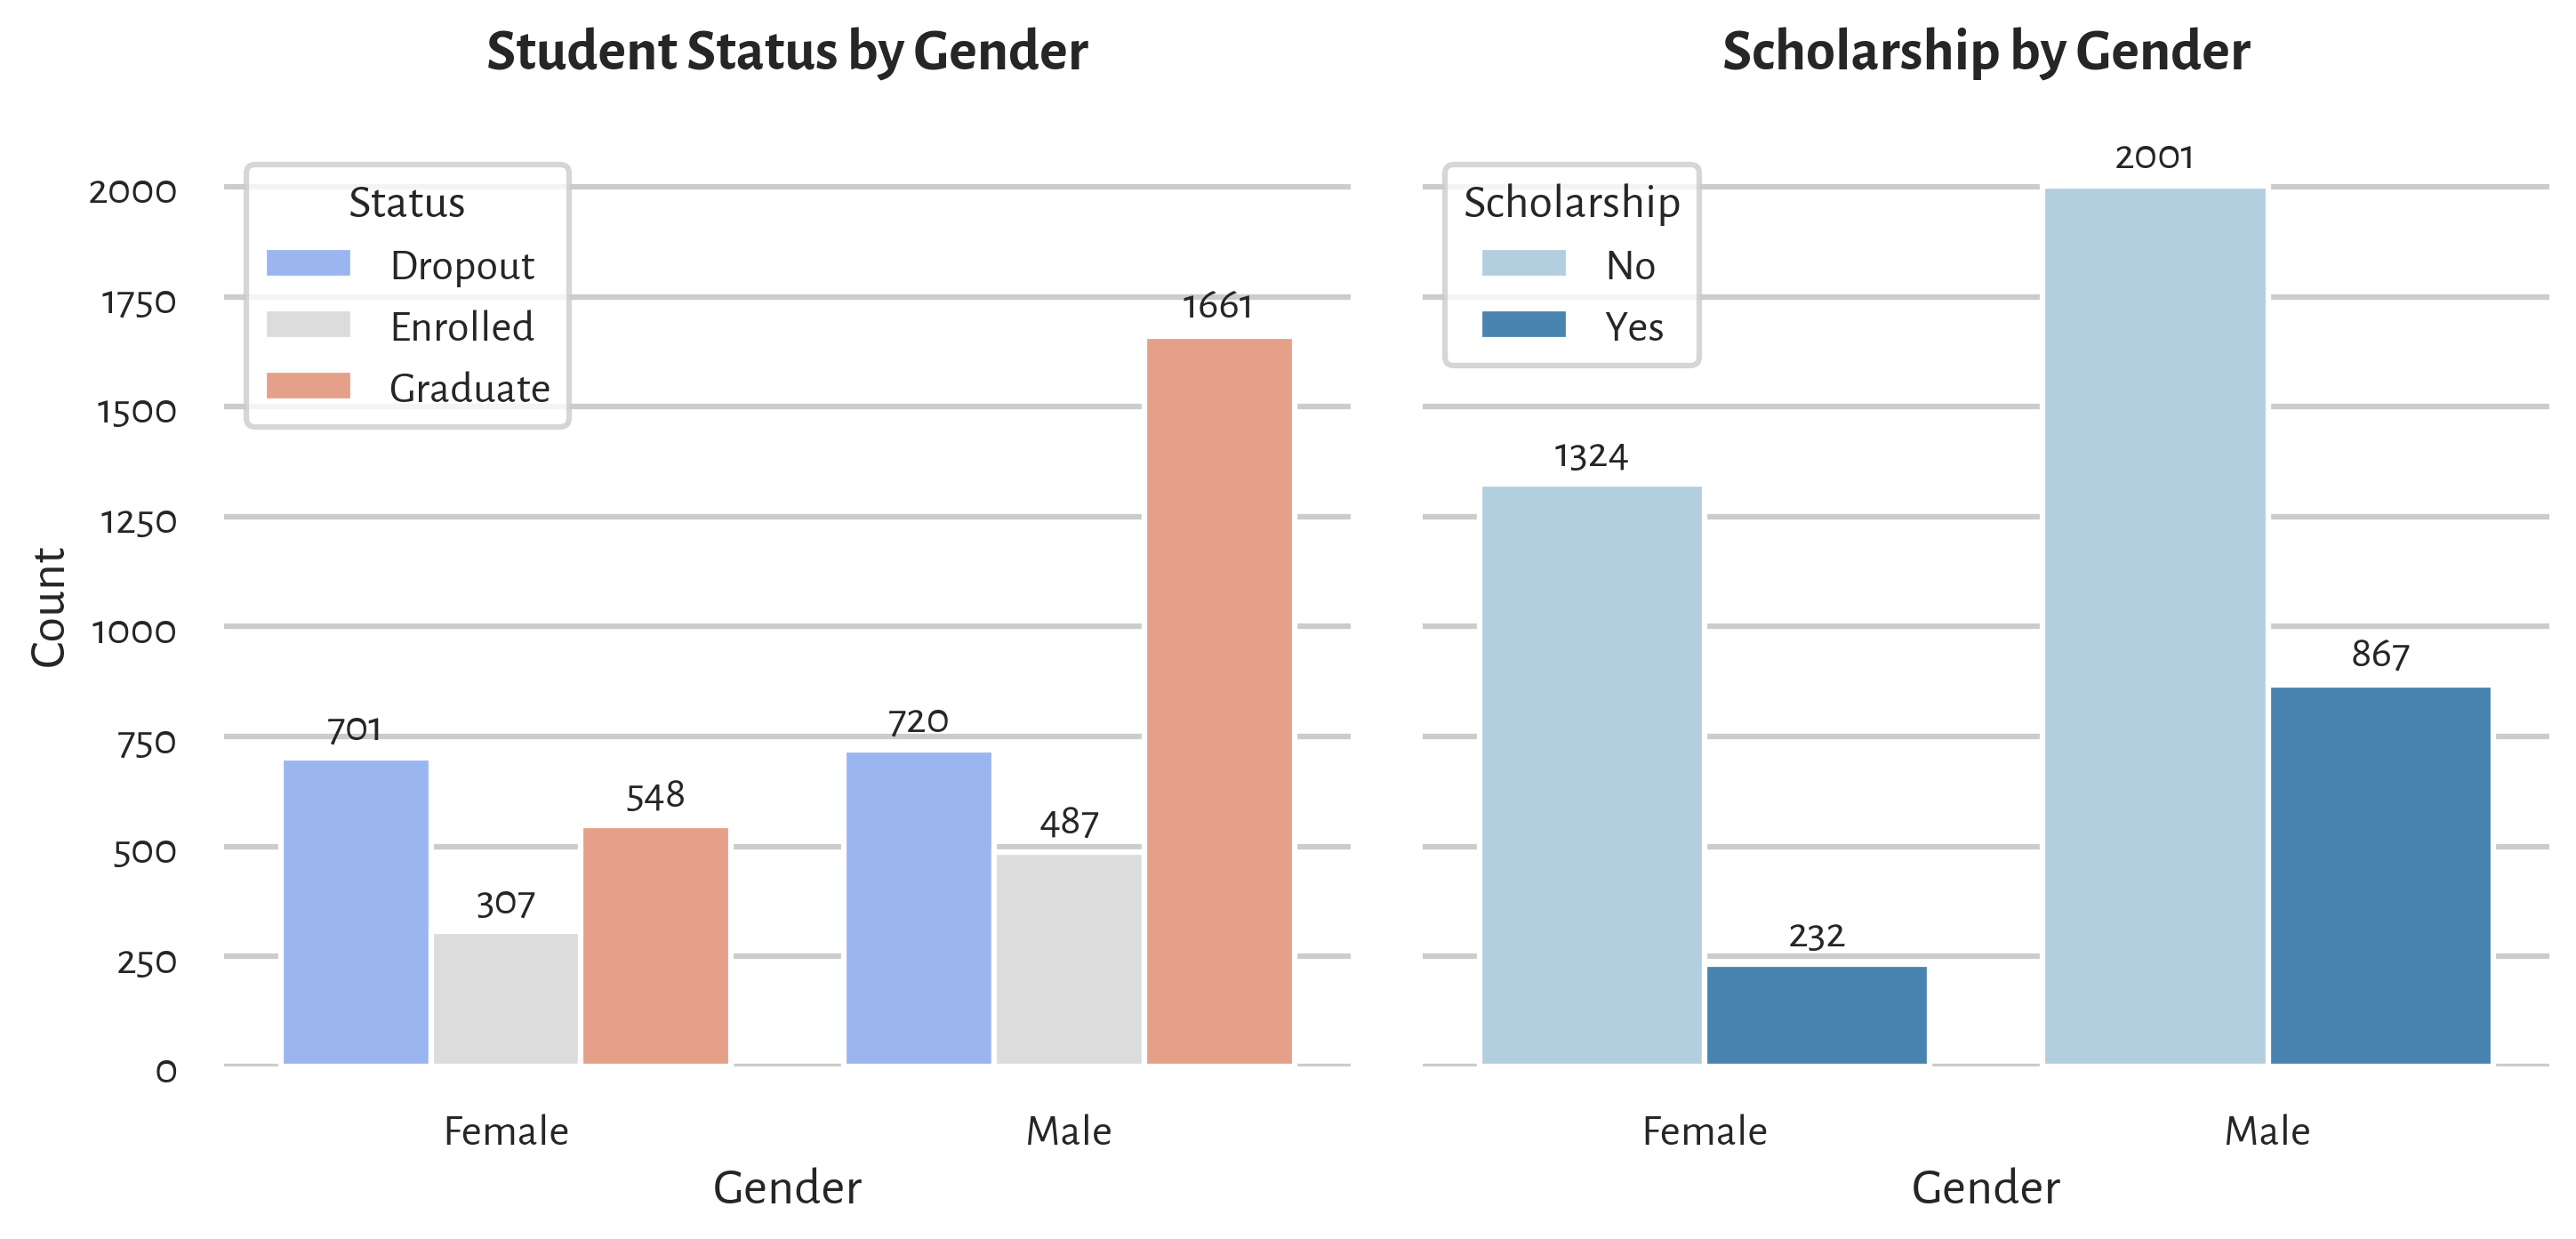
\includegraphics[width=1\textwidth]{Tex_Pictures/Graph_gender.png}
     \end{center}
\end{frame}

% ---------------------------------------
% Section Causal Graph and Covariate Selection
% ---------------------------------------

\section{4. Causal Graph and Covariate Selection}

\begin{frame}{Simplified Causal Graph}
	\begin{center}
     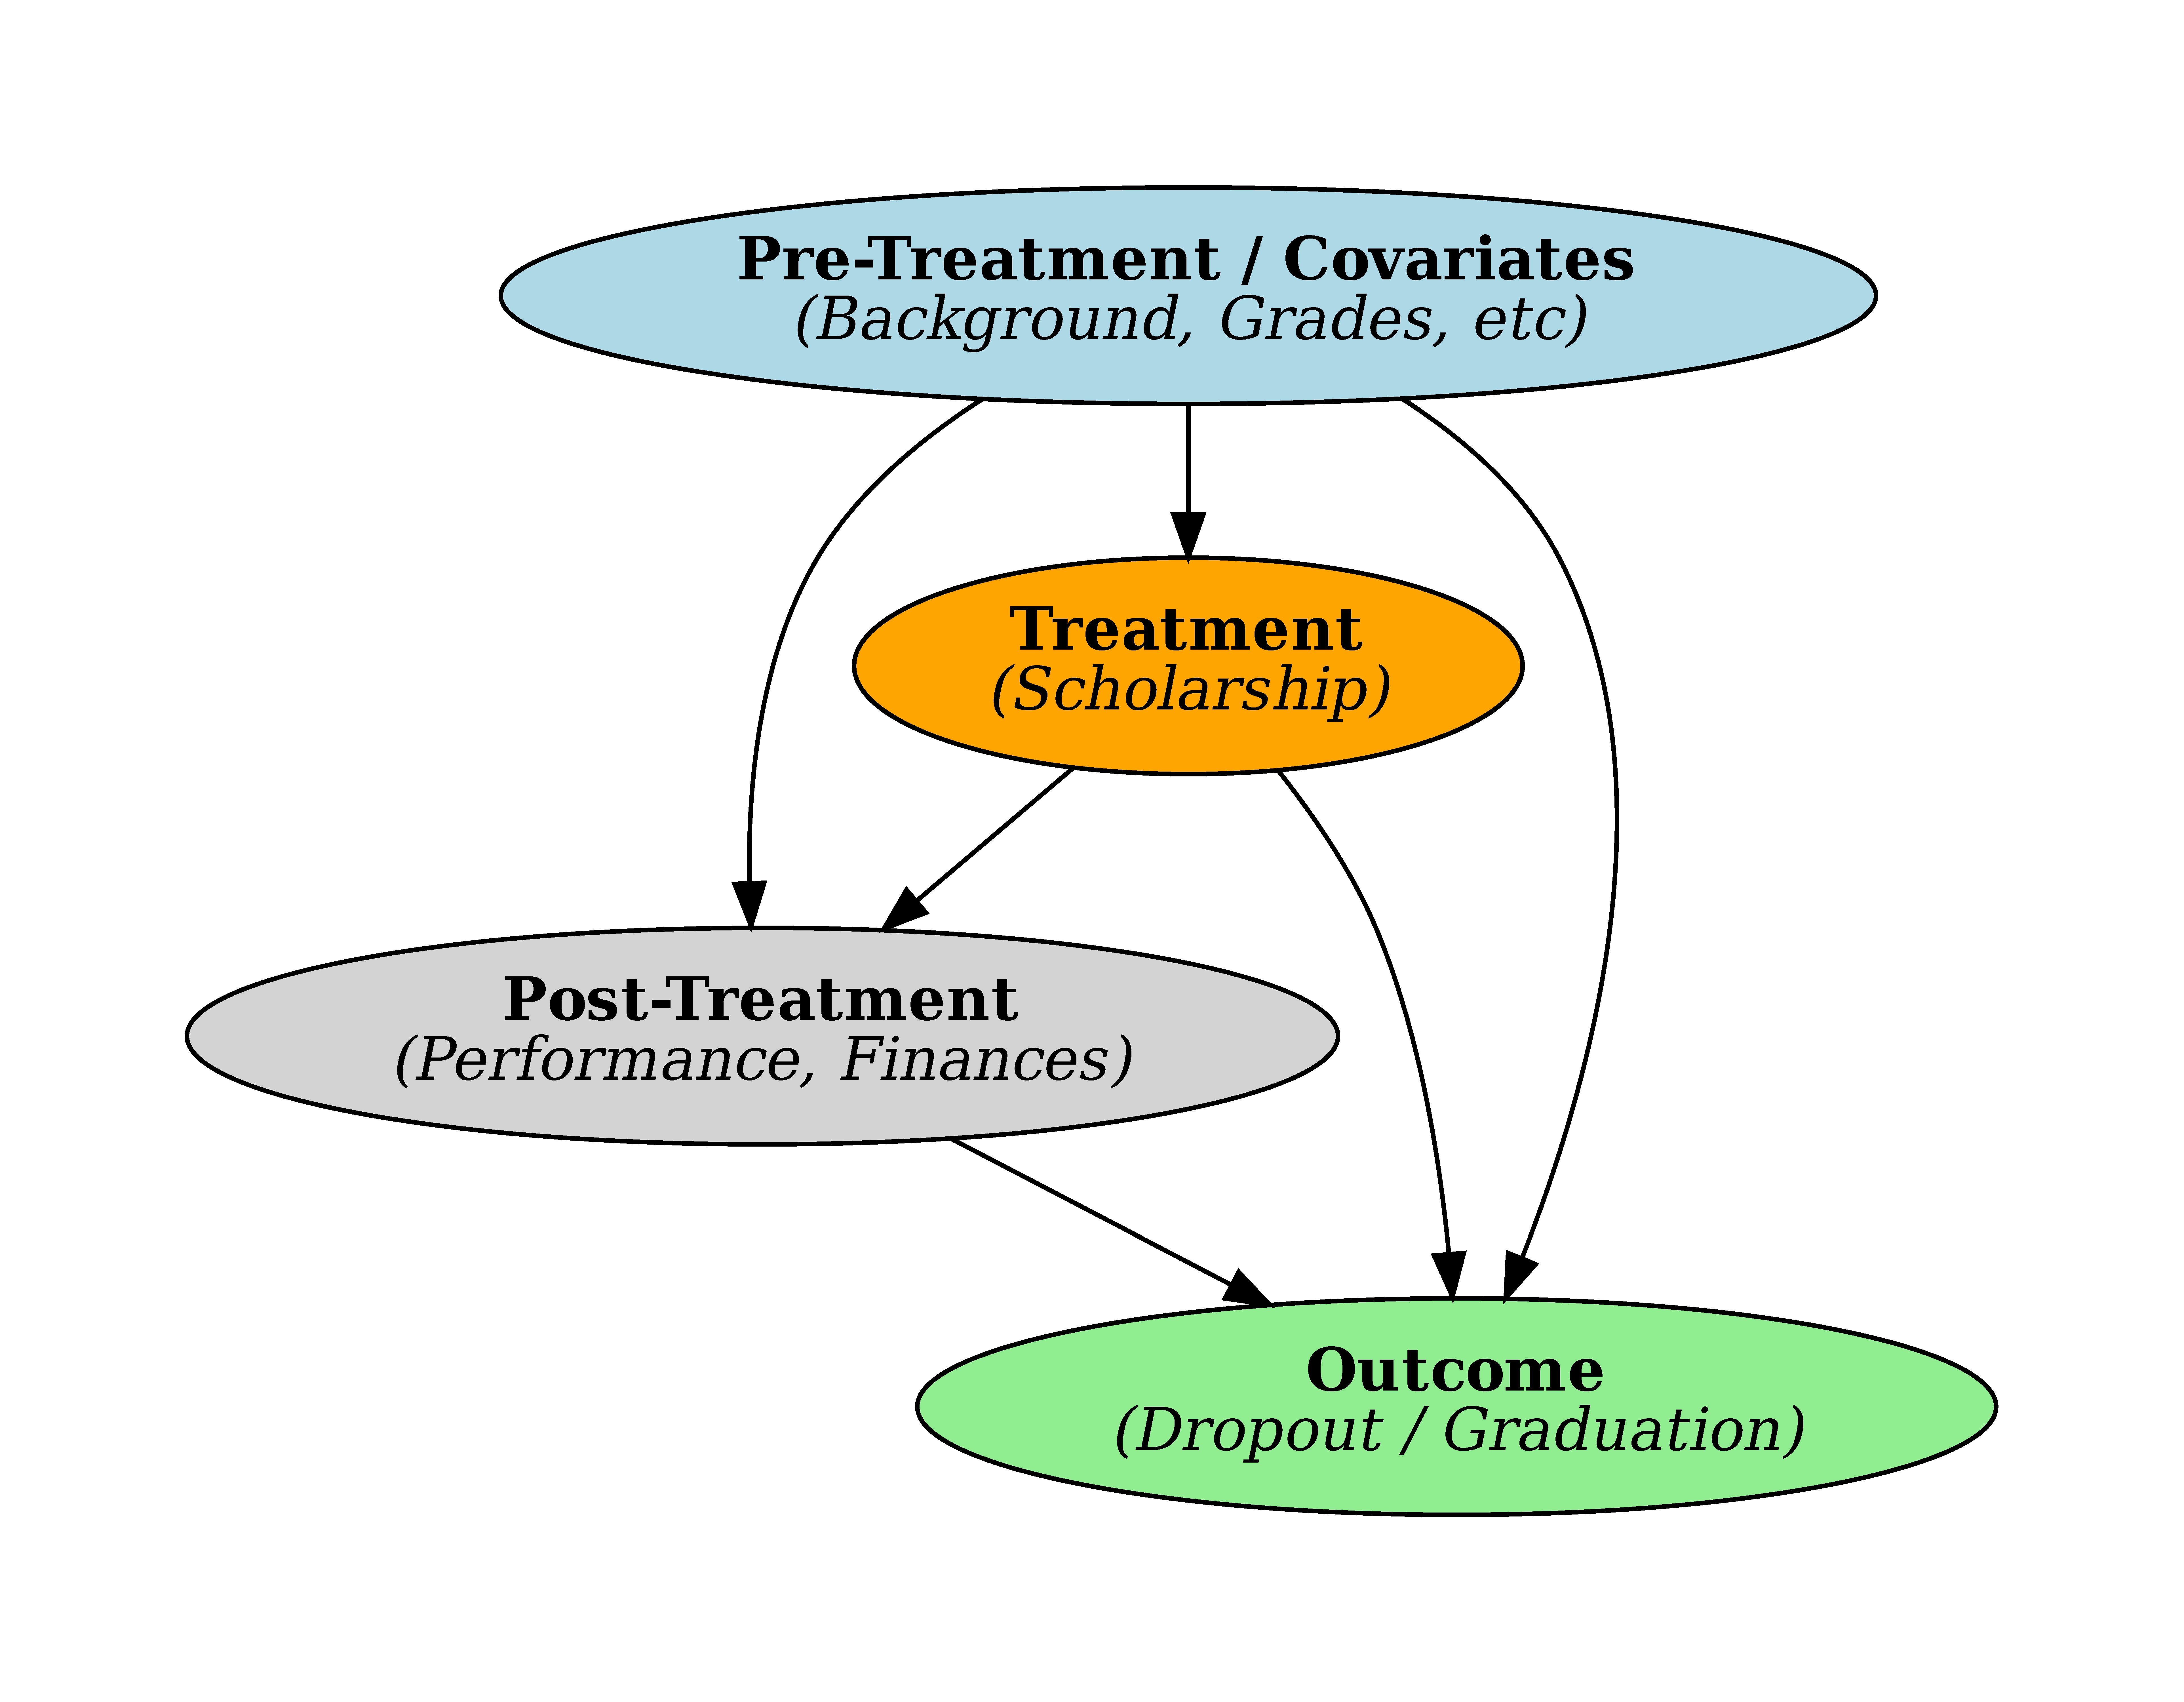
\includegraphics[width=0.6\textwidth]{Tex_Pictures/DAG_simple.png}
     \end{center}
\end{frame}

\begin{frame}{Simplified Causal Graph \& Relevant Paths}
	 \begin{columns}
	\begin{column}{0.58\textwidth}

\textbf{Three relevant paths between \\ Treatment (incoming) \& Outcome}
\small{
\begin{itemize}
    \item [1.] Treatment (incoming) $\leftarrow$ Covariates $\rightarrow$ Outcome
    \item [2.] Treatment (incoming) $\leftarrow$ Covariates $\rightarrow$ Post-Treatment $\rightarrow$ Outcome
    \item [3.] Treatment (incoming) $\leftarrow$ Covariates $\rightarrow$ Post-Treatment $\leftarrow$ Treatment (outgoing) $\rightarrow$ Outcome
\end{itemize}}
\begin{itemize}
	\item [$\Rightarrow$] All paths are blocked simultaneously by conditioning on the covariates, but NOT conditioning on the post-treatment effects.
\end{itemize}
  \end{column}

	\begin{column}{0.45\textwidth}
	\hspace*{-0.5cm}
    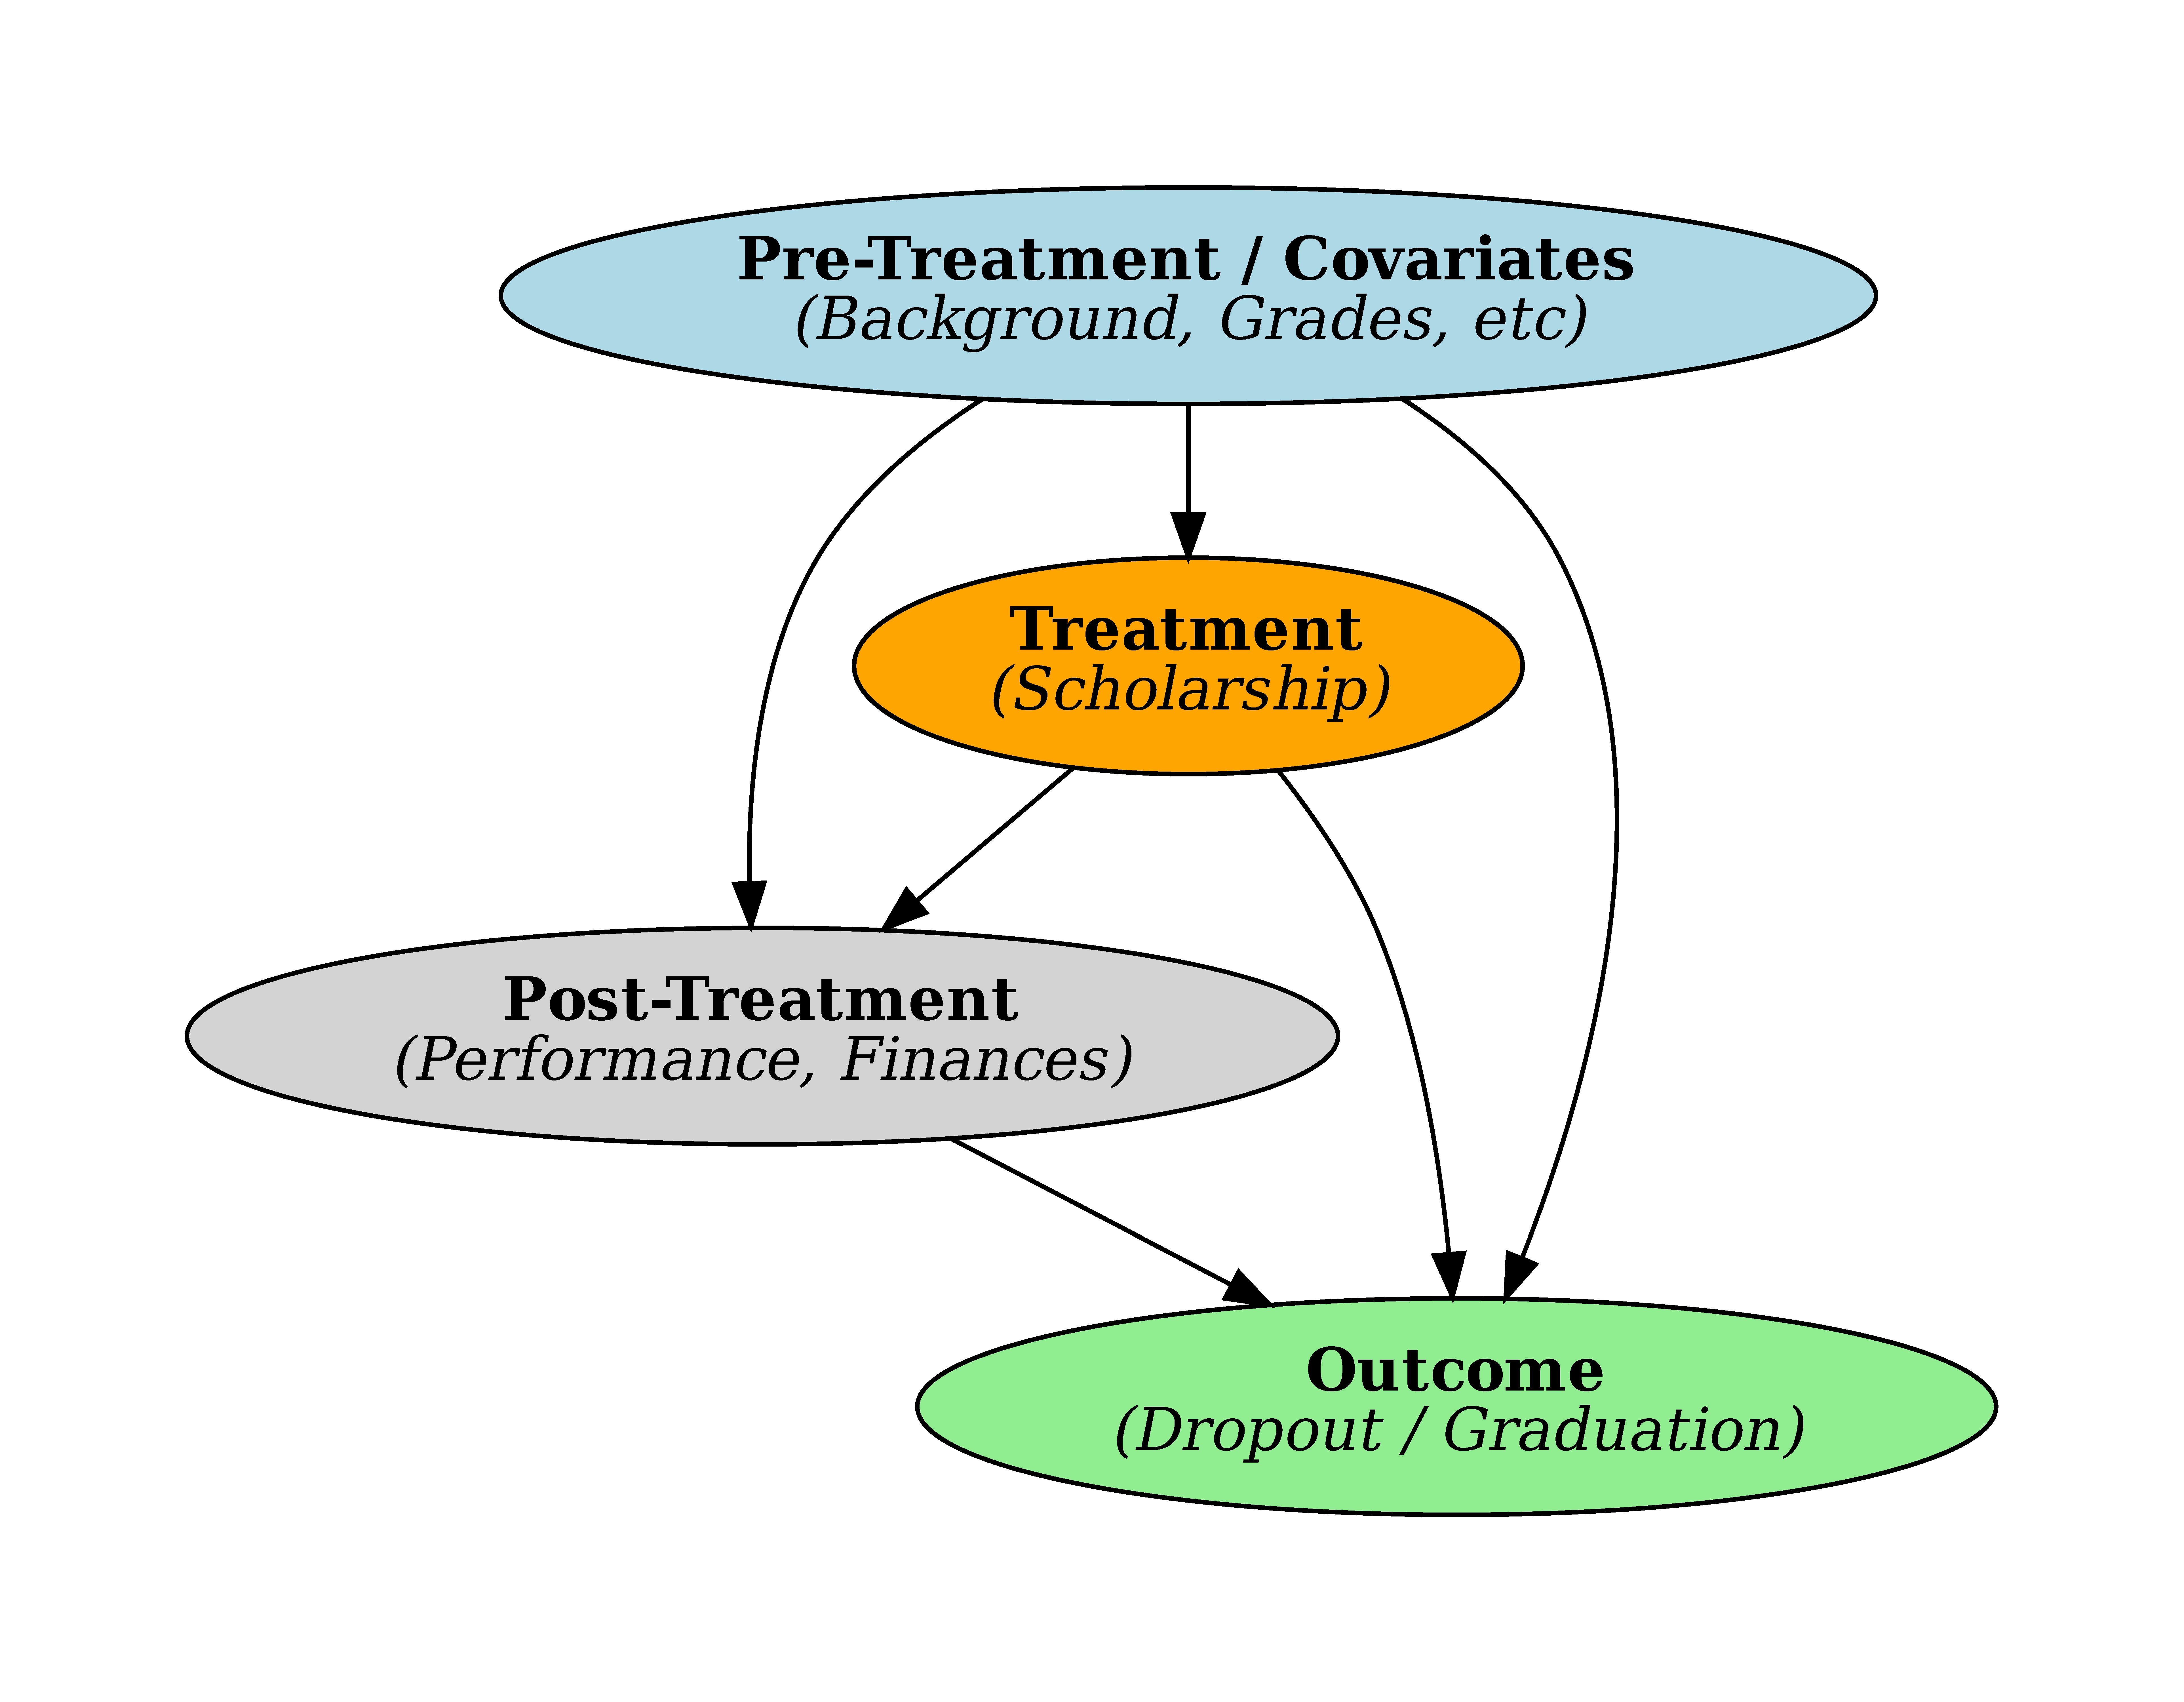
\includegraphics[width=1.1\textwidth]{Tex_Pictures/DAG_simple.png}

	\end{column}

\end{columns}
\end{frame}

\begin{frame}{Covariate selection}

	\textbf{37 features in the dataset, including one treatment and one target}
	\vspace{10pt}
	
	\begin{tabularx}{\textwidth}{X | X | X}
	\textbf{Pre-treatment (14)}  & \textbf{Post-treatment (14)} & \textbf{Unsuitable (7)} \\[0.5ex]
	\hline \hline 
	\parbox[t]{4cm}{\vspace{-12pt} \begin{itemize}
	[label=--,leftmargin=1.2em,itemsep=1pt,topsep=2pt]
    \item Academic performance before university
    \item Family background
    \item Economic context
    \item Individual characteristics (age, gender, etc.)
	\end{itemize}} 

	&
	\parbox[t]{4cm}{
	\vspace{-12pt}
	\begin{itemize}[label=--,leftmargin=1.2em,itemsep=1pt,topsep=2pt]
    	\item Academic performance during university
    	\item Financial situation during university
	\end{itemize}}
	&
	\parbox[t]{4cm}{\vspace{-12pt} 
	\begin{itemize}[label=--,leftmargin=1.2em,itemsep=1pt,topsep=2pt]
    	\item Marital status
    	\item Course selection
    	\item Parental occupation
    	\item Nationality
    	\item Etc.
	\end{itemize}} 
	\end{tabularx}


\end{frame}

\begin{frame}{Full Causal Graph}
	\begin{center}
	\textbf{Directed Acyclic Graph (DAG) of the Causal Relationships}
	\hspace*{-1cm}
     \includegraphics[width=1.15\textwidth]{Tex_Pictures/DAG_extended.png}
     \end{center}
\end{frame}

\begin{frame}{Assumptions}
\textbf{Main Assumptions for Identification of the Effect}
\begin{itemize}
    \item [1.] \textbf{Ignorability (Conditional Independence)}: \\No unmeasured factors that both influence scholarship status and dropout rate.
    \item [2.] \textbf{Positivity}: \\There should be an overlap in characteristics – for any combination of covariates, there are both scholarship and non-scholarship students.
    \item [3.] \textbf{No interference}: \\One student’s scholarship does not directly affect another’s outcome.
\end{itemize}

\end{frame}


% ---------------------------------------
% Section Double Post Lasso
% ---------------------------------------
\section{5. Causal Effect Estimation Using Double Post Lasso}

\begin{frame}{Results DPL: RQ1 (Dropout)}
\vspace{20pt}
    \begin{alertblock}{RQ1}
	Does receiving a scholarship \textbf{reduce} the likelihood of \textbf{dropping out} within 3 years?
	\end{alertblock}

\begin{block}{Results}
\begin{itemize}[label=--,itemsep=1pt,topsep=2pt]
	\item Covariates selected by Lasso: Outcome model - 4, Treatment model - 9
	\item Covariates in final union used for OLS: 10
	\item Estimated ATE of Scholarship on Dropout: -0.2030 (s.e. 0.0159) (p-value 0.0000***)
\end{itemize}
\end{block}

\begin{exampleblock}{Interpretation}
\vspace{-3pt}
\begin{itemize}
	\item [$\Rightarrow$]Receiving a scholarship \textit{significantly} \textbf{reduces} the probability of \textbf{dropout} within 3 years \\ by 20.3 \%-points. 
\end{itemize}
\vspace{-3pt}
\end{exampleblock}

\end{frame}

\begin{frame}{Results DPL: RQ2 (On-Time Graduation)}
\vspace{20pt}
\begin{alertblock}{RQ2}
	Does receiving a scholarship \textbf{increase} the likelihood of \textbf{graduating} within 3 years?
\end{alertblock}

\begin{block}{Results}
\begin{itemize}[label=--,itemsep=1pt,topsep=2pt]
	\item Covariates selected by Lasso: Outcome model - 10, Treatment model - 9
	\item Covariates in final union used for OLS: 12
	\item Estimated ATE of Scholarship on Graduation: -0.2789 (s.e. 0.0169) (p-value 0.0000***)
\end{itemize}
\end{block}

\begin{exampleblock}{Interpretation}
\vspace{-3pt}
\begin{itemize}
	\item [$\Rightarrow$]Receiving a scholarship \textit{significantly} \textbf{increases} the probability of \textbf{graduating} within \\ 3 years by 27.8 \%-points.
\end{itemize}
\vspace{-3pt}	
\end{exampleblock}

\end{frame}

% ---------------------------------------
% Section Double Machine Learning
% ---------------------------------------
\section{6. Causal Effect Estimation Using Double Machine Learning}

\begin{frame}{Steps (using all suitable covariates)}
\begin{itemize}
    \item [1.] Normalize numerical features
    \item[2.] Random forest classifier to model the treatment (who receives scholarships). It learns $P(T=1|X)$, the propensity score.
    \item [3.] Lasso regression with cross-validation, used to model the outcome $E[Y|X]$, i.e., the expected dropout probability given covariates.
    \item [4.] DoubleMLPLR (Partially Linear Regression) estimator for the causal effect of treatment on outcome, controlling for covariates.

\end{itemize}
    
\end{frame}
\begin{frame}{Results DML: RQ1 (Dropout)}
\vspace{20pt}
    \begin{alertblock}{RQ1}
	Does receiving a scholarship \textbf{reduce} the likelihood of \textbf{dropping out} within 3 years?
	\end{alertblock}

\begin{block}{Results}
\begin{itemize}[label=--,itemsep=1pt,topsep=2pt]
	\item Estimated Treatment Effect: -0.1701 (17\% decrease) (s.e. 0.0137)
	\item 95\% Confidence Interval: [-0.1969, -0.1432]
	\item P-value: 0.0000 (***) (t-stat: -12.4159)
\end{itemize}
\end{block}

\begin{exampleblock}{Interpretation}
\vspace{-3pt}
\begin{itemize}
	\item [$\Rightarrow$]Receiving a scholarship \textit{significantly} \textbf{reduces} the probability of \textbf{dropout} within 3 years \\ by 17.6 \%-points. 
\end{itemize}
\vspace{-3pt}
\end{exampleblock}

\end{frame}

\begin{frame}{Results DML: RQ2 (On-Time Graduation)}
\vspace{20pt}
\begin{alertblock}{RQ2}
	Does receiving a scholarship \textbf{increase} the likelihood of \textbf{graduating} within 3 years?
\end{alertblock}

\begin{block}{Results}
\begin{itemize}[label=--,itemsep=1pt,topsep=2pt]
	\item Estimated Treatment Effect: 0.2348 (23\% increase) (s.e. 0.0162)
	\item 95\% Confidence Interval: [0.2031, 0.2666]
	\item P-value: 0.0000 (***) (t-stat: 14.4859)
\end{itemize}
\end{block}

\begin{exampleblock}{Interpretation}
\vspace{-3pt}
\begin{itemize}
	\item [$\Rightarrow$]Receiving a scholarship \textit{significantly} \textbf{increases} the probability of \textbf{graduating} within \\ 3 years by 23.5 \%-points.
\end{itemize}
\vspace{-3pt}
	
\end{exampleblock}

\end{frame}

\section{7. Heterogenous treatment effects}



\begin{frame}{Gender-based Heterogeneity Analysis}
\vspace{5pt}
\begin{alertblock}{Approach}
	\textbf{Do scholarships affect male and female students differently?}
	\vspace{-10pt}
	\begin{itemize}[label=--,itemsep=1pt]
    \item Treatment effects estimated separately for male and female subgroups using DoubleML.
    \item Slightly stronger effects for female students across both outcomes.
\end{itemize}
\end{alertblock}
\vspace{5pt}
\begin{block}{Results}
\vspace{8}
\begin{columns}
\begin{column}{0.45\textwidth}
\textbf{RQ1 – Dropout (↓):}
\vspace{-3pt}
\begin{itemize}[label=--,itemsep=1pt]
    \item Males: \textbf{-0.1853 ± 0.0147}
    \item Females: \textbf{-0.2387 ± 0.0298}
\end{itemize}
\end{column}

\begin{column}{0.45\textwidth}
\textbf{RQ2 – Graduation (↑):}
\vspace{-3pt}
\begin{itemize}[label=--,itemsep=1pt]
    \item Males: \textbf{0.2630 ± 0.0180}
    \item Females: \textbf{0.2748 ± 0.0350}
\end{itemize}
\end{column}
\end{columns}
\vspace{4}
\end{block}



\vspace{5pt}
\begin{exampleblock}{Interpretation}
Scholarships \textbf{reduce dropout} and \textbf{improve graduation} outcomes for both genders, with a \textbf{slightly higher impact observed for female} students.

\end{exampleblock}

\end{frame}



\section{8. Robustness and Sensitivity Analysis}


\begin{frame}{Identifying Key Predictors of Student Outcomes using Feature Importance}
\textbf{Random Forest Feature Importance (Dropout and Scholarship Eligibility)}
\vspace{8pt}

\begin{columns}
\begin{column}{0.5\textwidth}
\centering
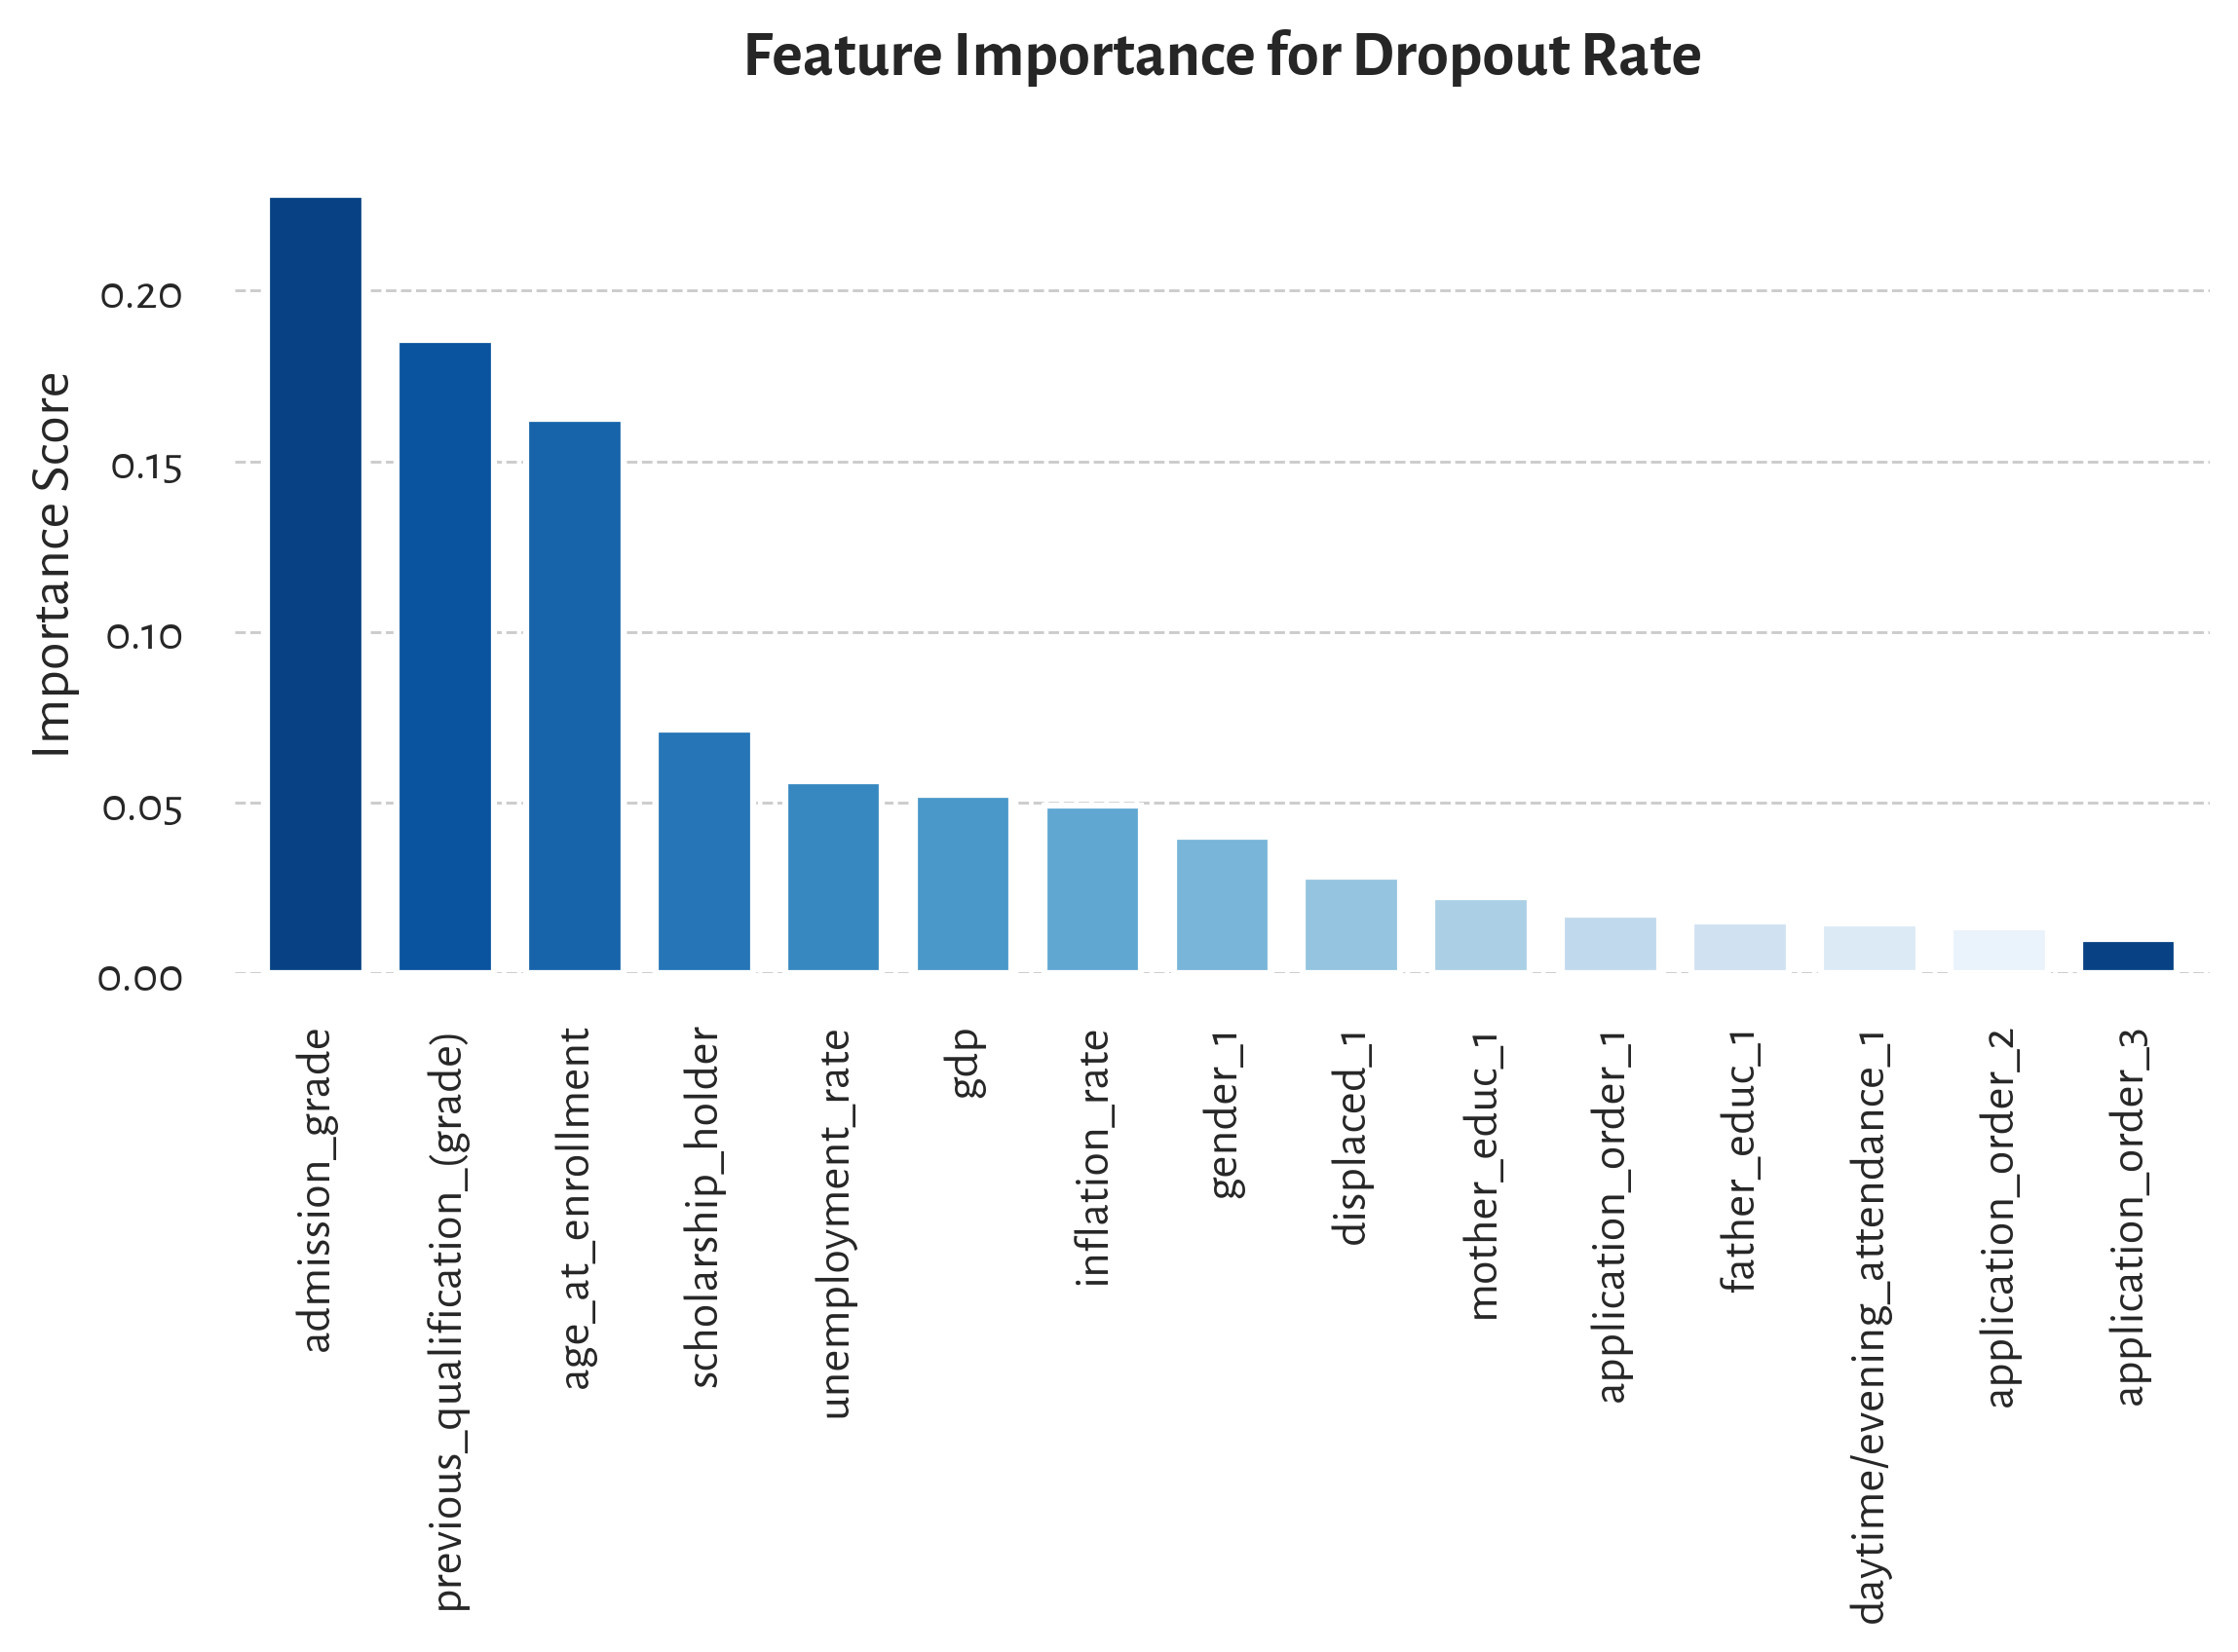
\includegraphics[width=\linewidth]{Tex_Pictures/feature_dropout.jpeg} \\
\small Dropout Prediction
\end{column}
\begin{column}{0.5\textwidth}
\centering
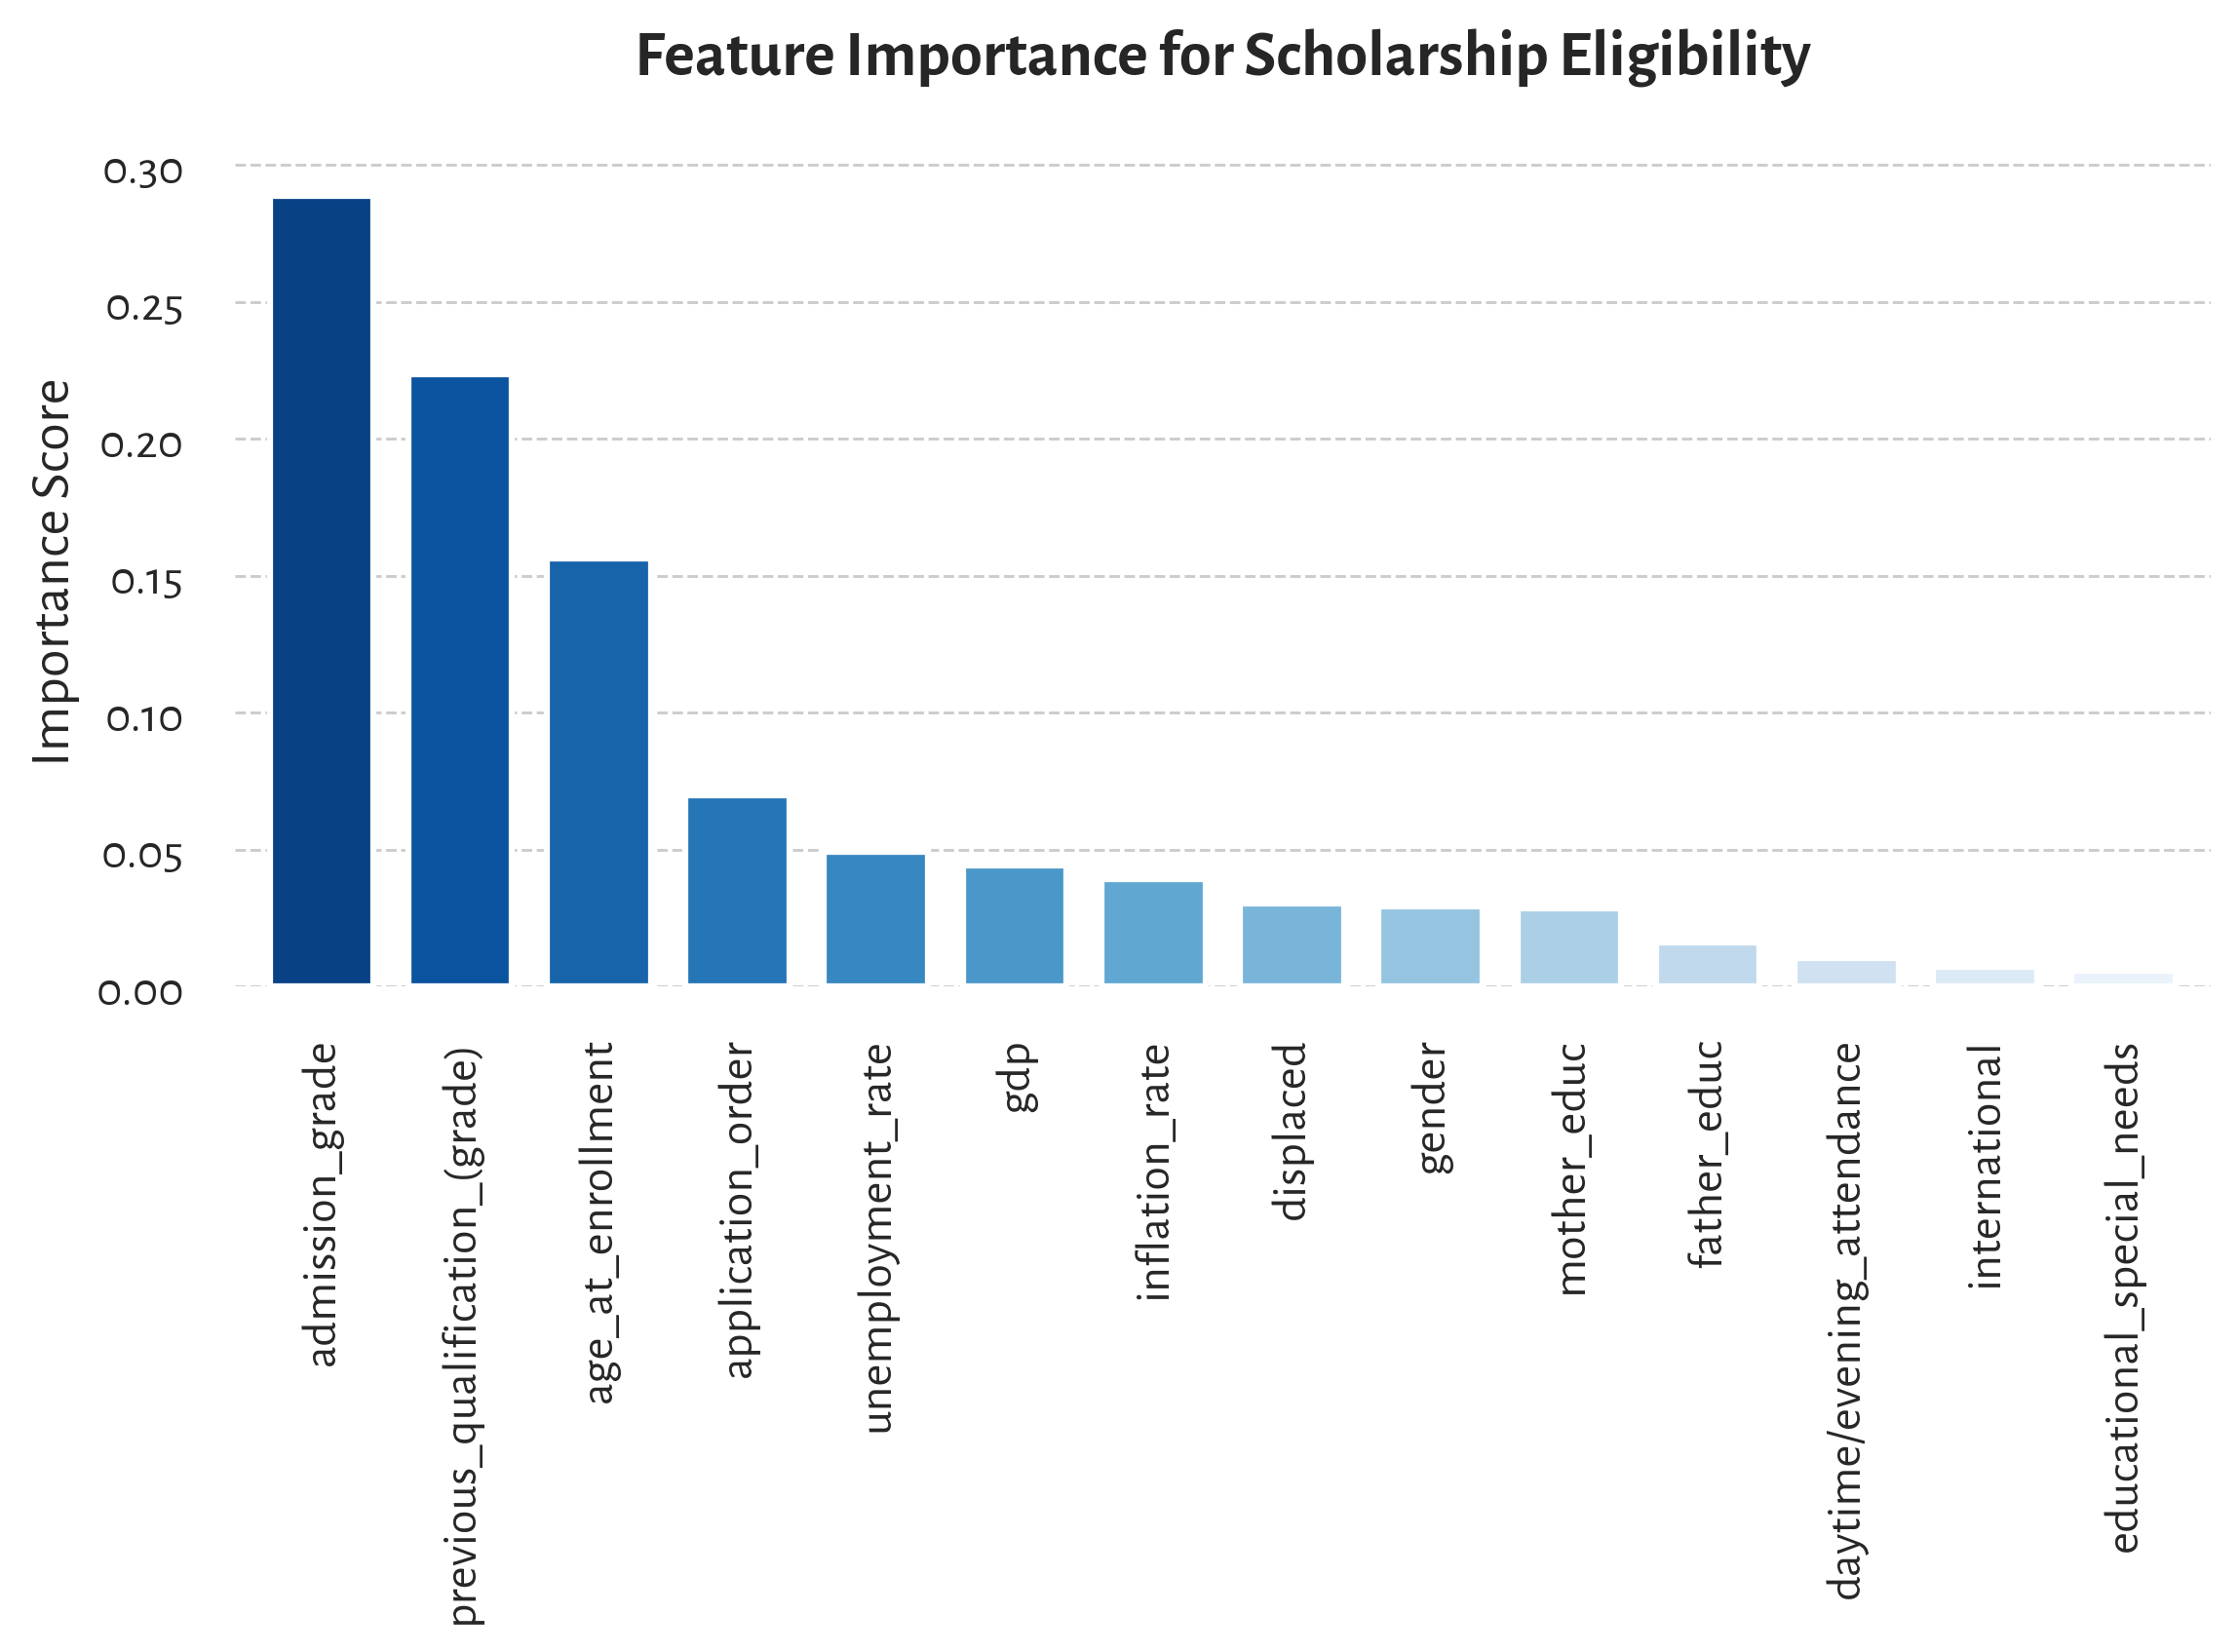
\includegraphics[width=\linewidth]{Tex_Pictures/feature_scholarship.jpeg} \\
\small Scholarship Eligibility
\end{column}
\end{columns}
\end{frame}

\begin{frame}{Identifying Key Predictors of Student Outcomes using Feature Importance}
\begin{block}{Feature Importance Analysis}
   
    The feature importance chart highlights academic performance (e.g., admission grades) as the strongest predictor of student outcomes. However, our primary variables of interest—\textbf{scholarship holding} and \textbf{gender}—appear less significant.
\end{block}


\begin{itemize}
    \item This is expected, as these variables likely affect student success \textit{indirectly}, mediated by academic factors and financial barriers.
    \item Random Forest prioritizes features that produce the best splits; hence, academic performance dominates.
    \item To assess \textbf{direct causal effects}, we exclude semester grades and proceed with causal inference models focused on scholarship and gender.
\end{itemize}
\end{frame}

\begin{frame}{Sensitivity Analysis: Covariate Sets}
\textbf{How robust are our results to different model specifications?}
\vspace{5pt}

We estimate the treatment effect using DoubleML while varying the covariates included in the model:

\begin{itemize}[label=--,itemsep=1pt]
    \item Academic preparation
    \item Family background
    \item Economic context
    \item Demographic controls (age, gender, etc.)
    \item Combined and full models
\end{itemize}

\vspace{5pt}
\textbf{Result:} The direction and significance of the effect remain stable, though the magnitude varies. The strongest effects are seen when economic and family background variables are included.
\end{frame}

\begin{frame}{Sensitivity Analysis: Visual}
\centering{
\textbf{Treatment effect estimates across different covariate sets.}}\\
\vspace{30pt}

\begin{columns}

\begin{column}{0.5\textwidth}
\centering
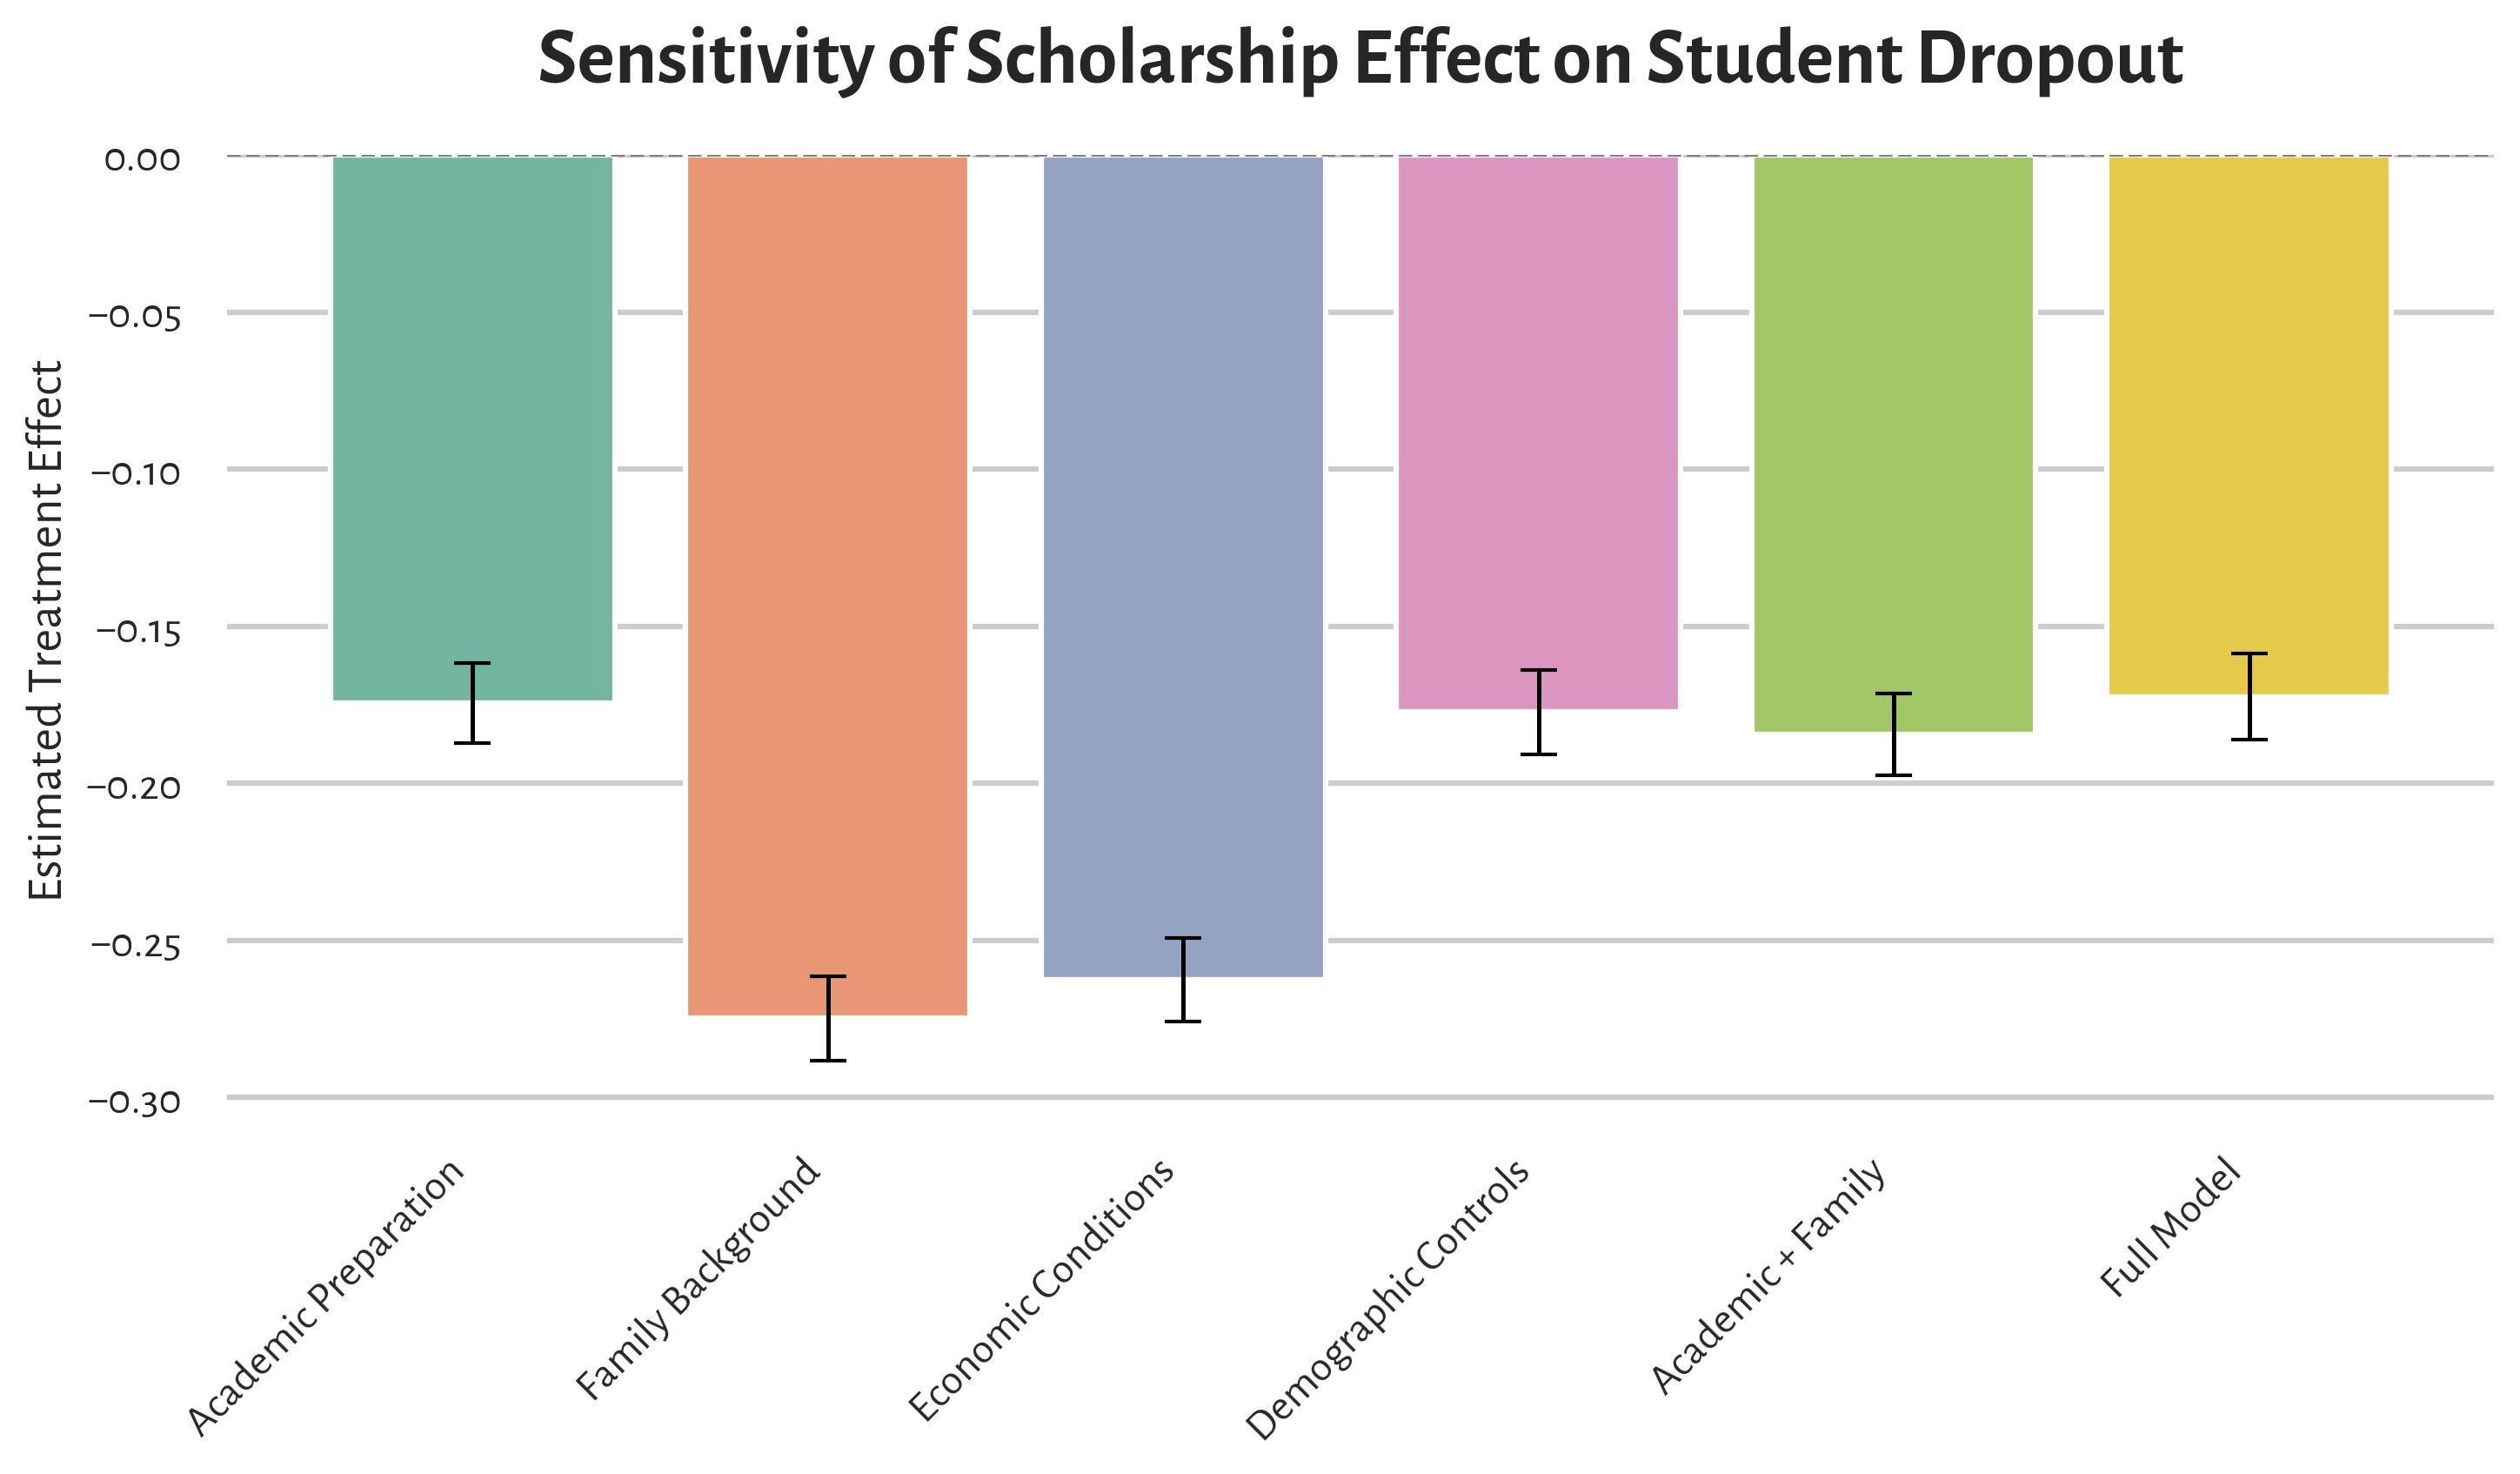
\includegraphics[width=1\linewidth]{Tex_Pictures/sensitivityrq1.png} \\
\small RQ1: Dropout
\end{column}
\begin{column}{0.5\textwidth}
\centering
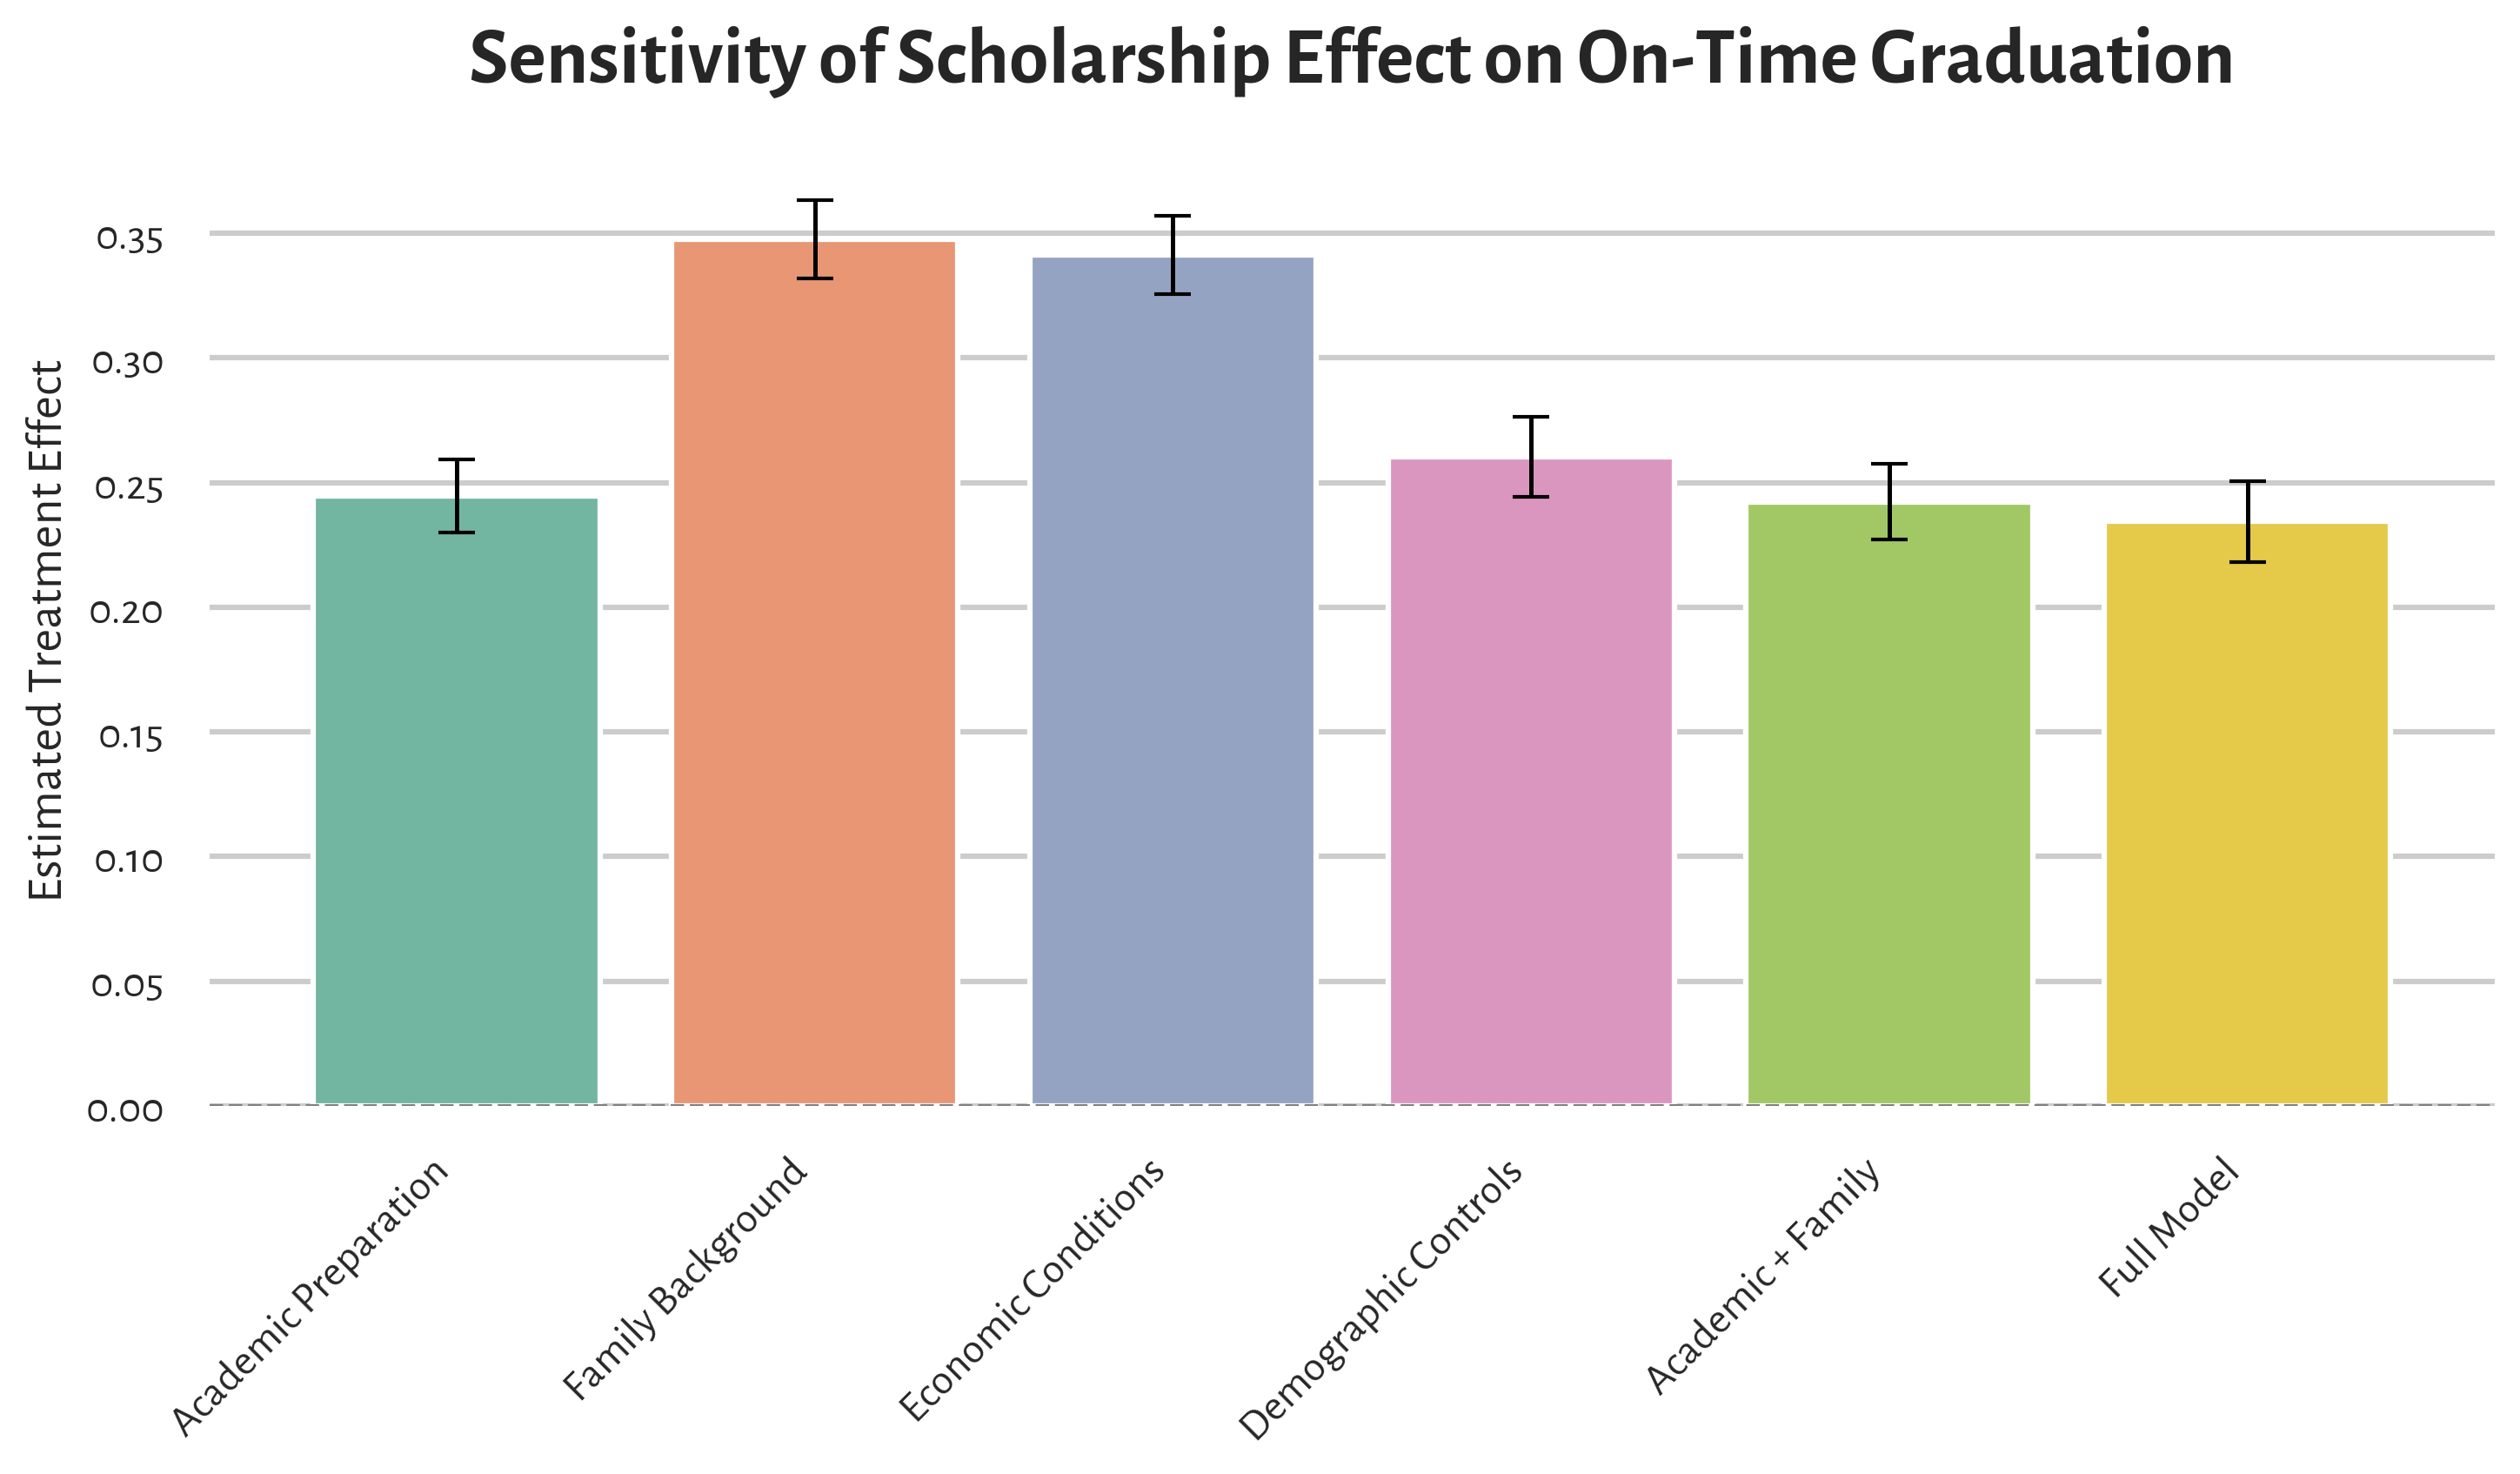
\includegraphics[width=1\linewidth]{Tex_Pictures/sensitivityrq2.png} \\
\small RQ2: On-Time Graduation
\end{column}
\end{columns}
\end{frame}



\begin{frame}{Placebo Test (RQ1 \& RQ2)}
\textbf{What if scholarship assignments were random?}
\vspace{10pt}

\begin{itemize}[label=--,itemsep=1pt]
    \item We randomly permute the treatment variable (scholarship).
    \item Re-run DML using this randomized “placebo” treatment.
    \item Expectation: no causal effect should be detected.
\end{itemize}

\vspace{10pt}
\textbf{Result:} Estimated placebo effects for both dropout and graduation are close to zero and statistically insignificant.

\vspace{5pt}
$\Rightarrow$ Supports that original results are unlikely to be due to spurious correlation or overfitting.
\end{frame}


\begin{frame}{Robustness Summary}
\begin{itemize}[label=--,itemsep=1pt]
    \item Treatment effects are statistically significant and stable across covariate sets.
    \item Stronger effects seen for students from lower socio-economic backgrounds.
    \item No significant treatment effect detected in placebo test $\rightarrow$ supports causal interpretation.
\end{itemize}

\vspace{10pt}
\begin{block}{Conclusion}
Our results are robust to model specification and randomization checks, suggesting that scholarships have a genuine causal impact on student success.
\end{block}

\end{frame}

\section{X. Conclusion}

  
\end{document}